\chapter{Teoría de los sistemas MIMO}

En términos generales, se puede definir a un sistema MIMO (multiple input multiple output) como un sistema caracterizado por poseer múltiples entradas y salidas. Debido a la abstracción de esta definición, la misma puede ajustarse a distintos campos de estudio. El tema que se abordará será el estudio de sistemas MIMO en las radiocomunicaciones, en las cuales se trabajará con señales que provienen de ondas electromagnéticas. 

En este caso particular de comunicaciones, los sistemas MIMO se refieren a sistemas que poseen múltiples antenas para captar señales en la entrada y múltiples antenas para transmitir las señales de salida.

\begin{figure}[htb!]
        \centering
        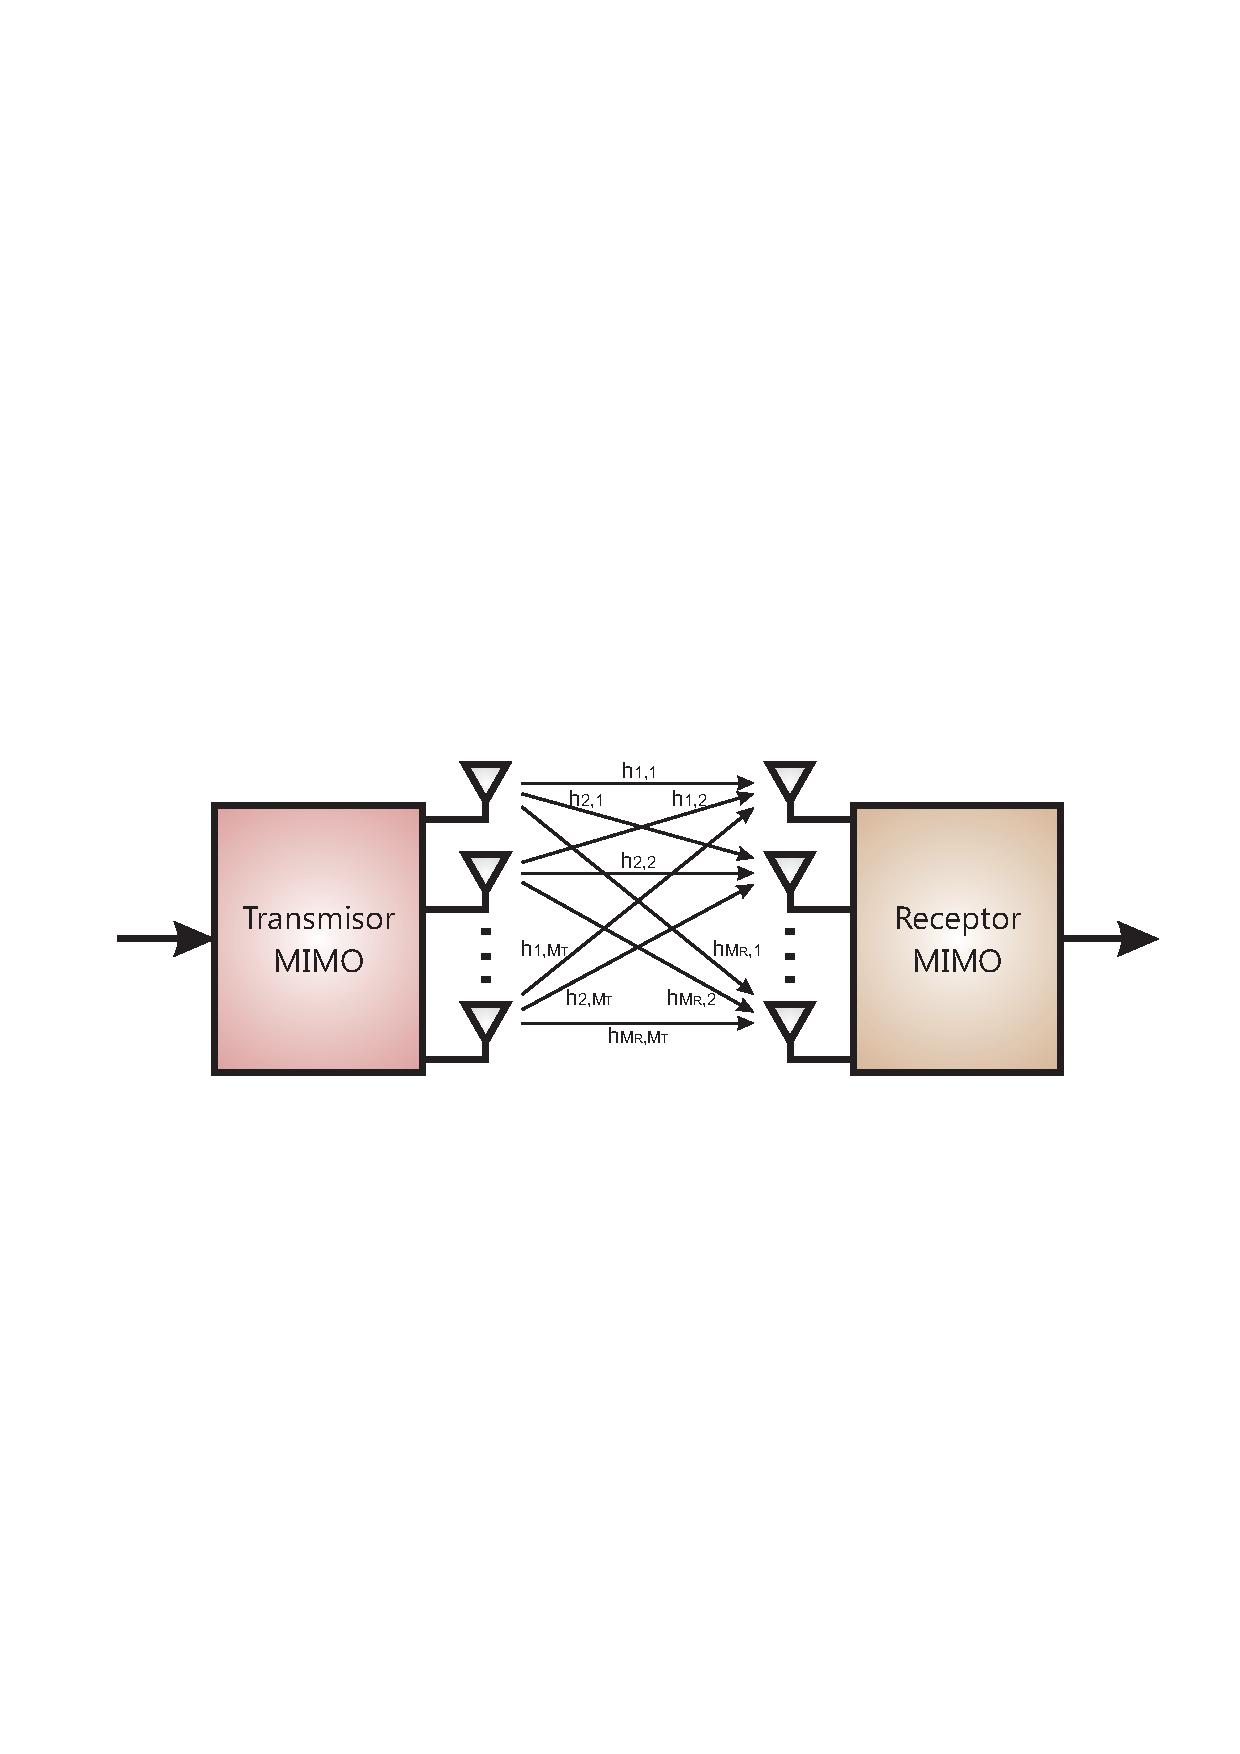
\includegraphics[width=11cm]{./figures/C02-MIMO_diagram_01}
        \caption{Esquema de un sistema de comunicación MIMO}
        \label{fig:MIMO_diagram_01}
\end{figure}

Una comunicación inalámbrica se compone por tres elementos. Un transmisor, un receptor, y el canal, en el cual se propagan las señales a transmitir/recibir \cite{Mohammadi}. Existe una clasificación para los distintos tipos de sistemas MIMO en función de la cantidad de antenas que poseen en los lados emisor y receptor. MIMO propiamente dicho, se refiere a un sistema en el cual se tiene más de una única antena tanto en el receptor como en el emisor del sistema. Los sistemas en los cuales se tiene una única antena en el receptor y múltiples antenas en el transmisor son conocidos como MISO (multiple input single output). Por otro lado, los sistemas SIMO (single input multiple output), son aquellos en los cuales se tiene una única antena en el lado emisor y múltiples antenas en el lado receptor. SISO (single input single output) es el caso en el cual se tiene una única antena tanto en la entrada como en la salida.

\begin{figure}[htb!]
        \centering
        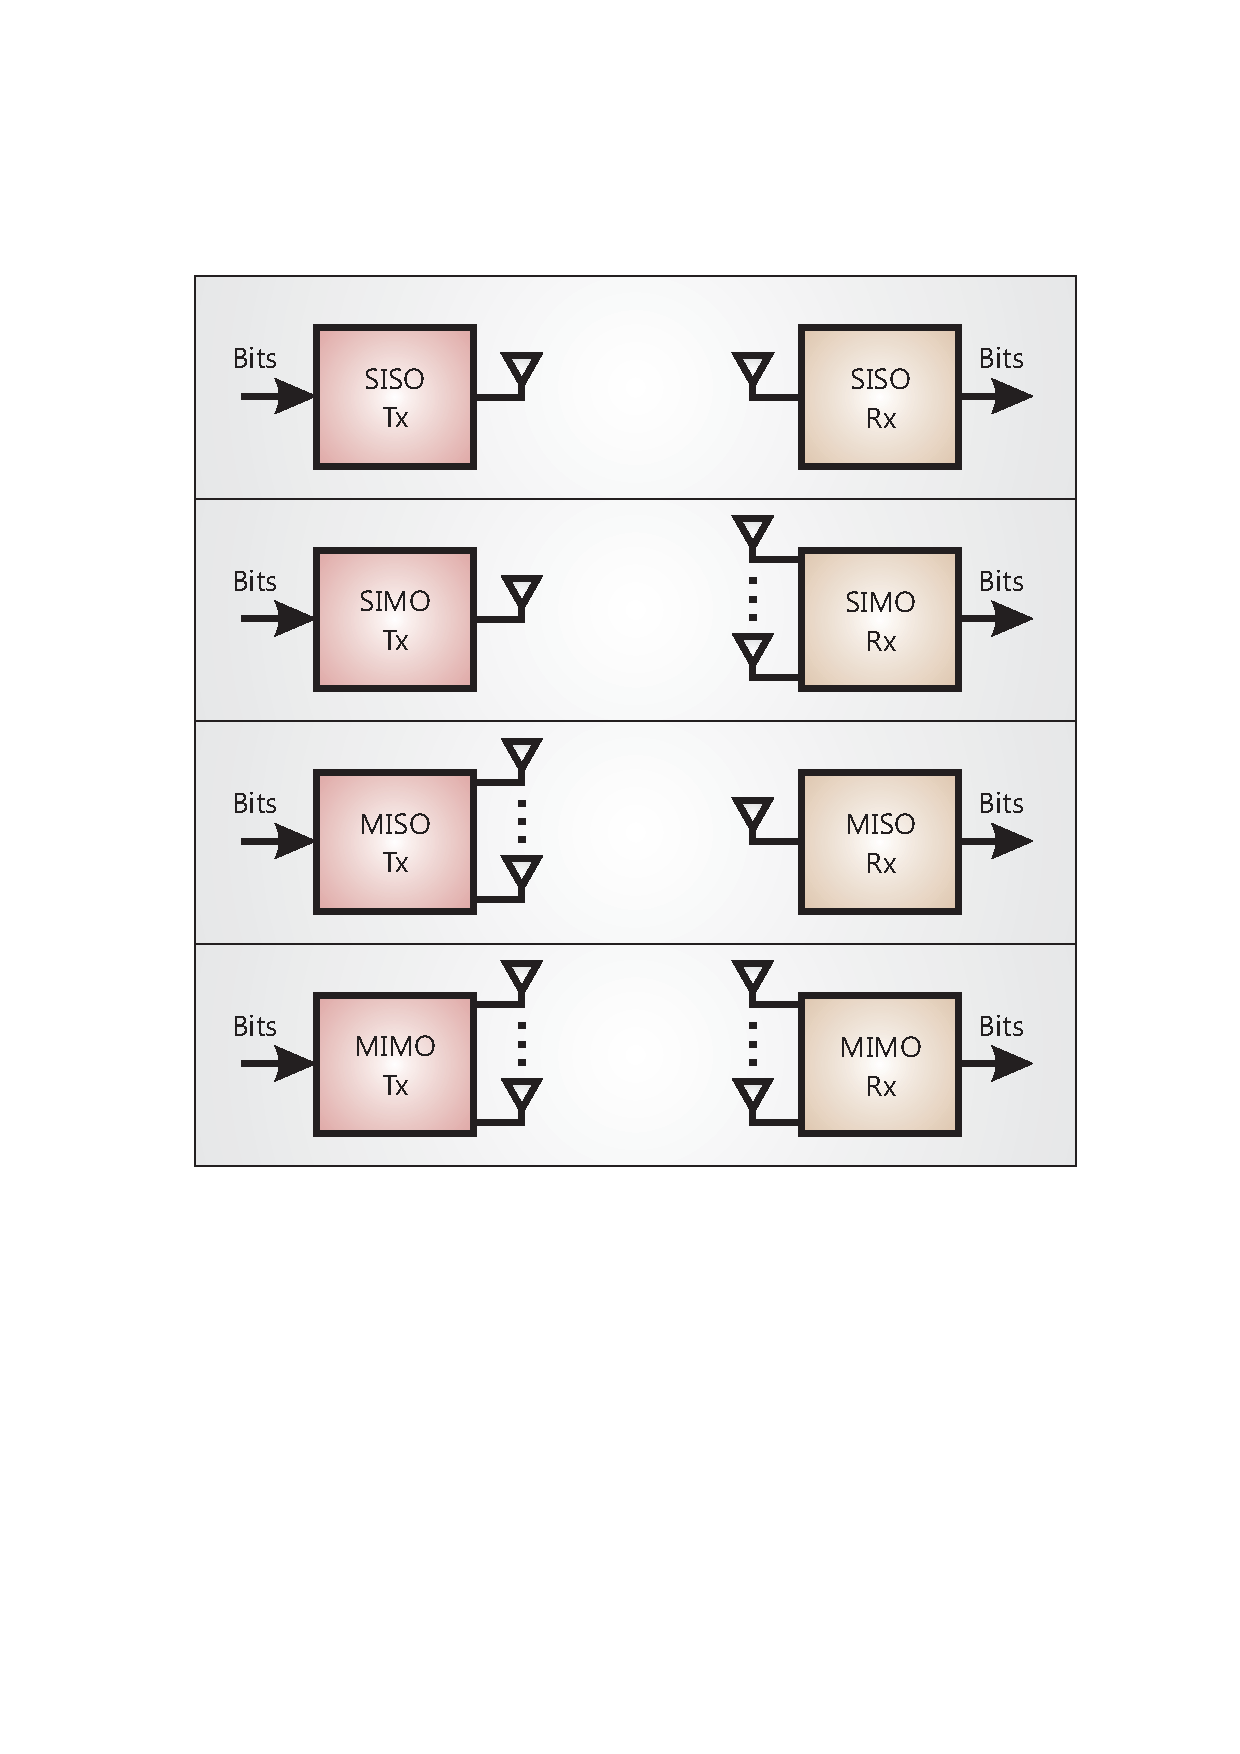
\includegraphics[width=8cm]{./figures/C02-MIMO_Combinations}
        \caption{Representación de los distintos sistemas de múltiples antenas}
        \label{fig:MIMO_Combinations}
\end{figure}

El concepto de utilizar múltiples antenas en un receptor de comunicaciones inalámbricas surgió en 1960. La idea escencial consistía en la provisión de múltiples copias de una señal transmitida en el lado receptor y sus combinaciones para obtener una señal de mejor desempeño \cite{Mohammadi}. Ésta técnica, es conocida como \textbf{diversidad espacial}. Para lograr la técnica de diversidad espacial, se emplean múltiples antenas en el lado receptor. Las señales de las antenas de salida son luego combinadas aplicando distintos coeficientes de ponderación. Por otro lado, el estudio de la implementación de diversidad a través de múltiples antenas en el lado transmisor fue introducido en 1990 \cite{Paulraj}. 

A través de la utilización de múltiples antenas es posible lograr una mayor eficiencia en distintas características de un sistema de comunicación, siendo las más importantes el aumento en la capacidad del canal o en la relación señal ruido. También es posible resolver conflictos vinculados a distintos fenómenos asociados con una comunicación inalámbrica. Uno de estos fenómenos es el conocido como \textbf{\textit{``Multipath Fading''}}. Antes de abordar dicho fenómeno se hará una breve reseña de algunos conceptos sobre antenas.

\section{Antenas}

Una antena es un dispositivo eléctrico que convierte potencia eléctrica en ondas de radio, y viceversa. Usualmente, es utilizada con un radio transmisor o radio receptor. En una transmisión, el transmisor de radio provee una corriente eléctrica oscilante de radio frecuencia a las terminales de la antena, y la misma irradia la energía proveniente de dicha corriente como ondas electromagnéticas (ondas de radio). En la recepción, una antena intercepta parte de la potencia de una onda electromagnética con el objetivo de producir un voltaje muy pequeño en sus terminales, el cual es aplicado al receptor para luego ser amplificado \cite{Wiki_Antenna}.

La antena consiste de conductores eléctricos (cables, tubos o superficies reflectantes) que crean campos eléctricos y magnéticos en el espacio alrededor de los mismos. \cite{Haynes}. Si los campos son variantes, se propagan hacia el espacio como ondas electromagnéticas a la velocidad de la luz:

\begin{equation}
\text{Velocidad de la Luz} \qquad  c \approx 3 \cdot 10^8 \frac{metros}{seg}
\end{equation}

Toda antena que transmite también recibe. Las ondas electromagnéticas que atraviesan la misma excitan corrientes en los conductores de la antena. La antena captura parte de la energía de las ondas que la atraviesan y la convierte en señales eléctricas en el cable.

Al realizarse el diseño de una antena, sus dimensiones son especificadas en términos de la longitud de onda de las señales de radio que serán transmitidas o recibidas. La longiud de onda es la distancia desde el inicio de un ciclo electromagnético hasta el próximo.

\begin{equation}
\lambda = \frac{c}{f_c}
\end{equation}

$\lambda$ es la longitud de onda en metros y $f_c$ es la frecuencia portadora de señal de radio en $Hz$. c es la velocidad de la luz ($3 \cdot 10^8 metros/seg$).


\begin{table}[htb!]
    \begin{center}
        \begin{tabular}{|c|c|c|}
        \hline  
        \textbf{Señal} & \textbf{Frecuencia} & \textbf{Longitud de Onda} \\
        \hline  
        Radio AM & $1 MHz$ & 300 metros \\
        \hline
        Radio FM & $100 MHz$ & 3 metros \\
        \hline
        Teléfono Celular & $850 MHz$ & 35 centímetros \\
        \hline
        Access Point Wi-Fi & $2,4 GHz$ & 12,5 centímetros \\
        \hline
        \end{tabular}
        \caption{Ejemplos de bandas de frecuencias y sus longitudes de onda}
    \end{center}
\end{table}


\subsection{Patrón de radiación de una antena}

Una antena transmisora genera ondas electromagnéticas más fuertes en algunas direcciones con respecto a otras. Para analizar este comportamiento se obtiene un diagrama de intensidad del campo en función de la dirección, el cual es llamado ``Patrón de radiación de la antena''. Siempre es igual para la recepción y para la transmisión.

Una onda electromagnética medida en un punto lejos de la antena es la suma de la radiación de todas las partes de la antena. Cada parte de la misma, irradia ondas de diferentes amplitudes y fases, y cada una de esos ondas viaja distintas distancias hasta el punto donde se encuentra el receptor. En algunas direcciones, estas ondas se suman constructivamente para dar una ganancia. En otras, se suman destructivamente para dar una pérdida.

Un dipolo de media onda es una antena simple que consiste de media longitud de onda de cable, cortado en el centro para realizar la conexión. En la siguiente figura se muestra su patrón de radiación:

\begin{figure}[htb!]
        \centering
        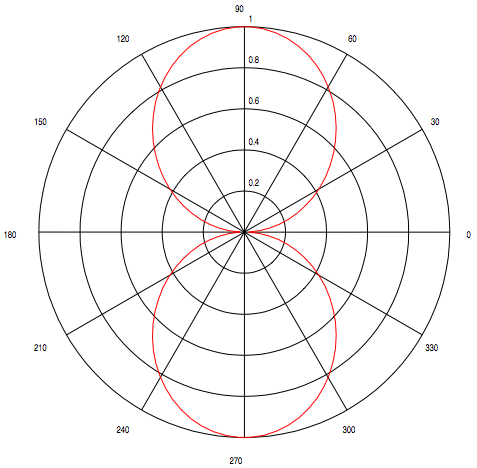
\includegraphics[width=6cm]{./figures/C02-half_wave_dipole}
        \caption{Dipolo de media onda - Intensidad de Campo vs Dirección}
        \label{fig:half_wave_dipole}
\end{figure}

\begin{figure}[htb!]
        \centering
        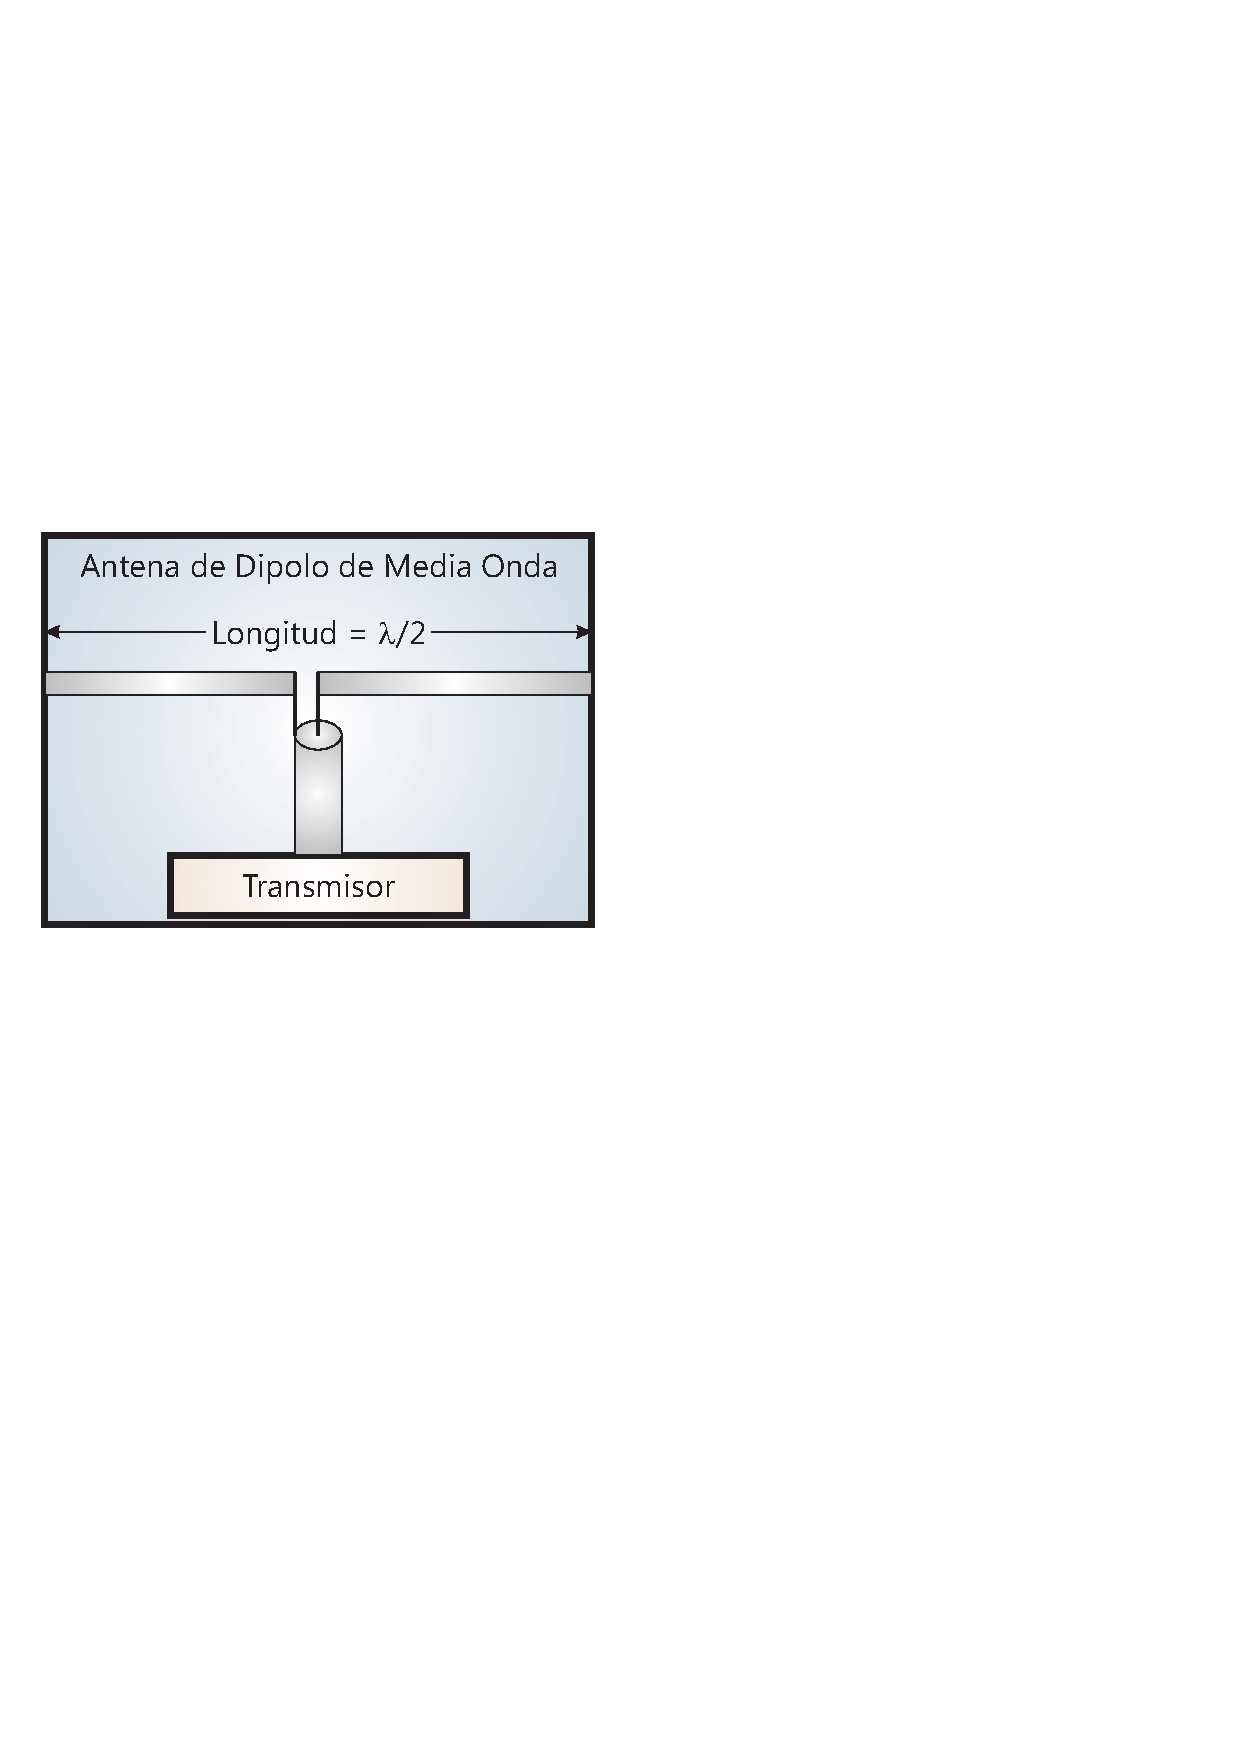
\includegraphics[width=6cm]{./figures/C02-half_wave_dipole_2}
        \caption{Dipolo de media onda - Esquema}
        \label{fig:half_wave_dipole_2}
\end{figure}

\subsection{Antenas direccionales}

Un ejemplo de antena direccional es una antena diseñada para tener ganancia en una dirección y pérdida en otras. Una antena se vuelve direccional al aumentar su tamaño. Al hacer esto, se amplian los conductores radiantes de la antena para cubrir una distancia mayor, de forma tal que las interferencias constructivas y destructivas pueden ser controladas de mejor forma para dar un patrón de radiación direccional.

Una antena de plato satelital puede ser considerada, simplisticamente, una superficie circular que irradia ondas electromagnéticas igualmente desde todas partes. Tiene un haz central angosto de alta ganancia, como se muestra en la siguiente figura, que se apunta al satélite.

A medida que se incrementa el diametro del plato en longitudes de onda, el haz central se vuelve más angosto. Notar los lóbulos pequeños, llamados ``lóbulos laterales'', a cada lado del haz central. Las direcciones en las cuales la intensidad de señal es cero son llamadas `nulls''.

\begin{figure}[htb!]
        \centering
        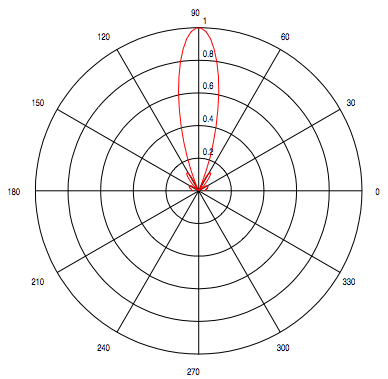
\includegraphics[width=6cm]{./figures/C02-dish_antenna}
        \caption{Antena Parabólica - Patrón de Radiación}
        \label{fig:dish_antenna}
\end{figure}

\begin{figure}[htb!]
        \centering
        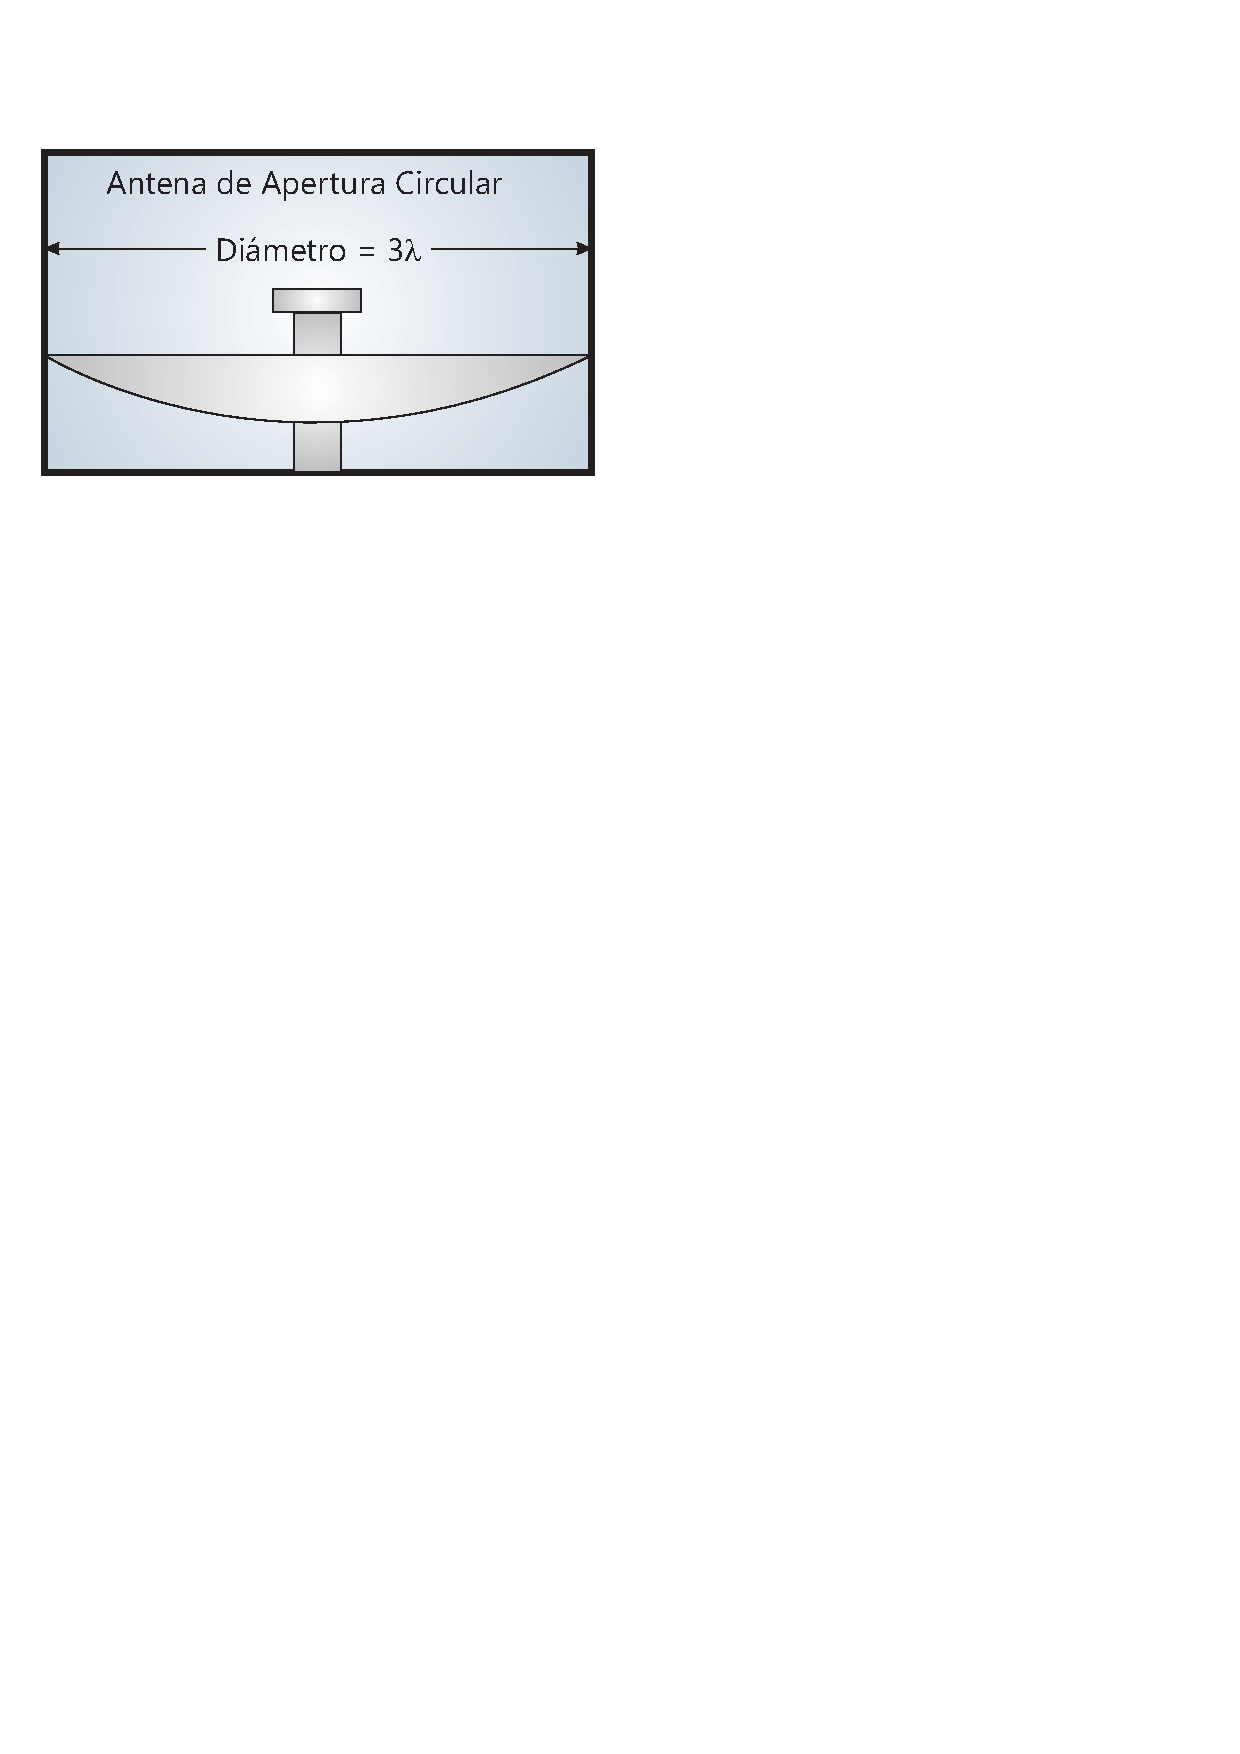
\includegraphics[width=6cm]{./figures/C02-dish_antenna_2}
        \caption{Antena Parabólica - Diagrama}
        \label{fig:dish_antenna_2}
\end{figure}

\subsection{Arreglos lineales}

Una antena direccional simple consiste de un arreglo lineal de pequeños elementos radiantes de antena, cada uno alimentado con señales idénticas (misma amplitud y fase) desde un transmisor. A medida que el ancho total del arreglo crece, el haz central se vuelve más angosto. A medida que el número de elementos se incrementa, los lóbulos laterales se vuelven más pequeños.

La siguiente figura es el patrón de raciación para una linea de 4 elementos (antenas pequeñas) espaciadas $1/2$ longitud de onda.

\begin{figure}[htb!]
        \centering
        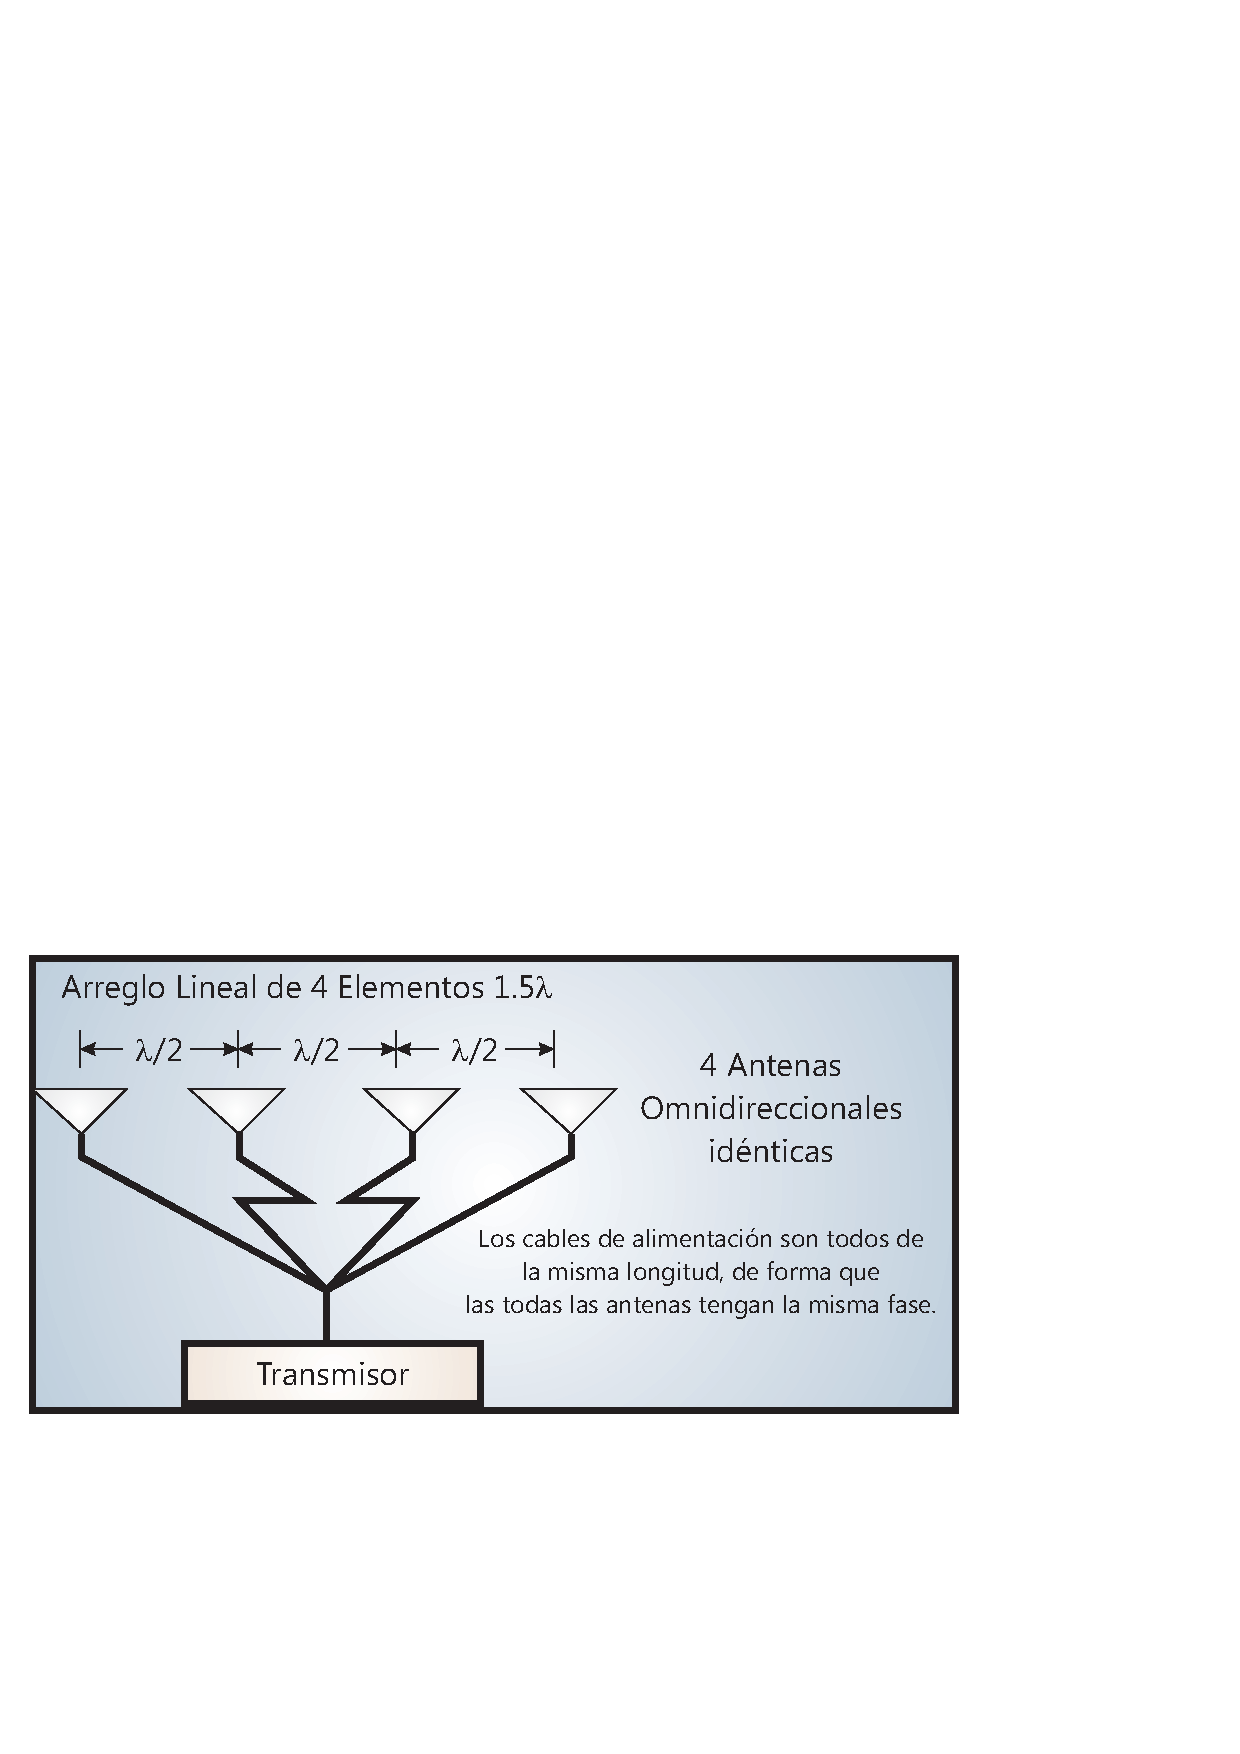
\includegraphics[width=7cm]{./figures/C02-linear_array_1}
        \caption{Arreglo Lineal $D=\lambda/2$ - Patrón de Radiación}
        \label{fig:linear_array_1}
\end{figure}

\begin{figure}[htb!]
        \centering
        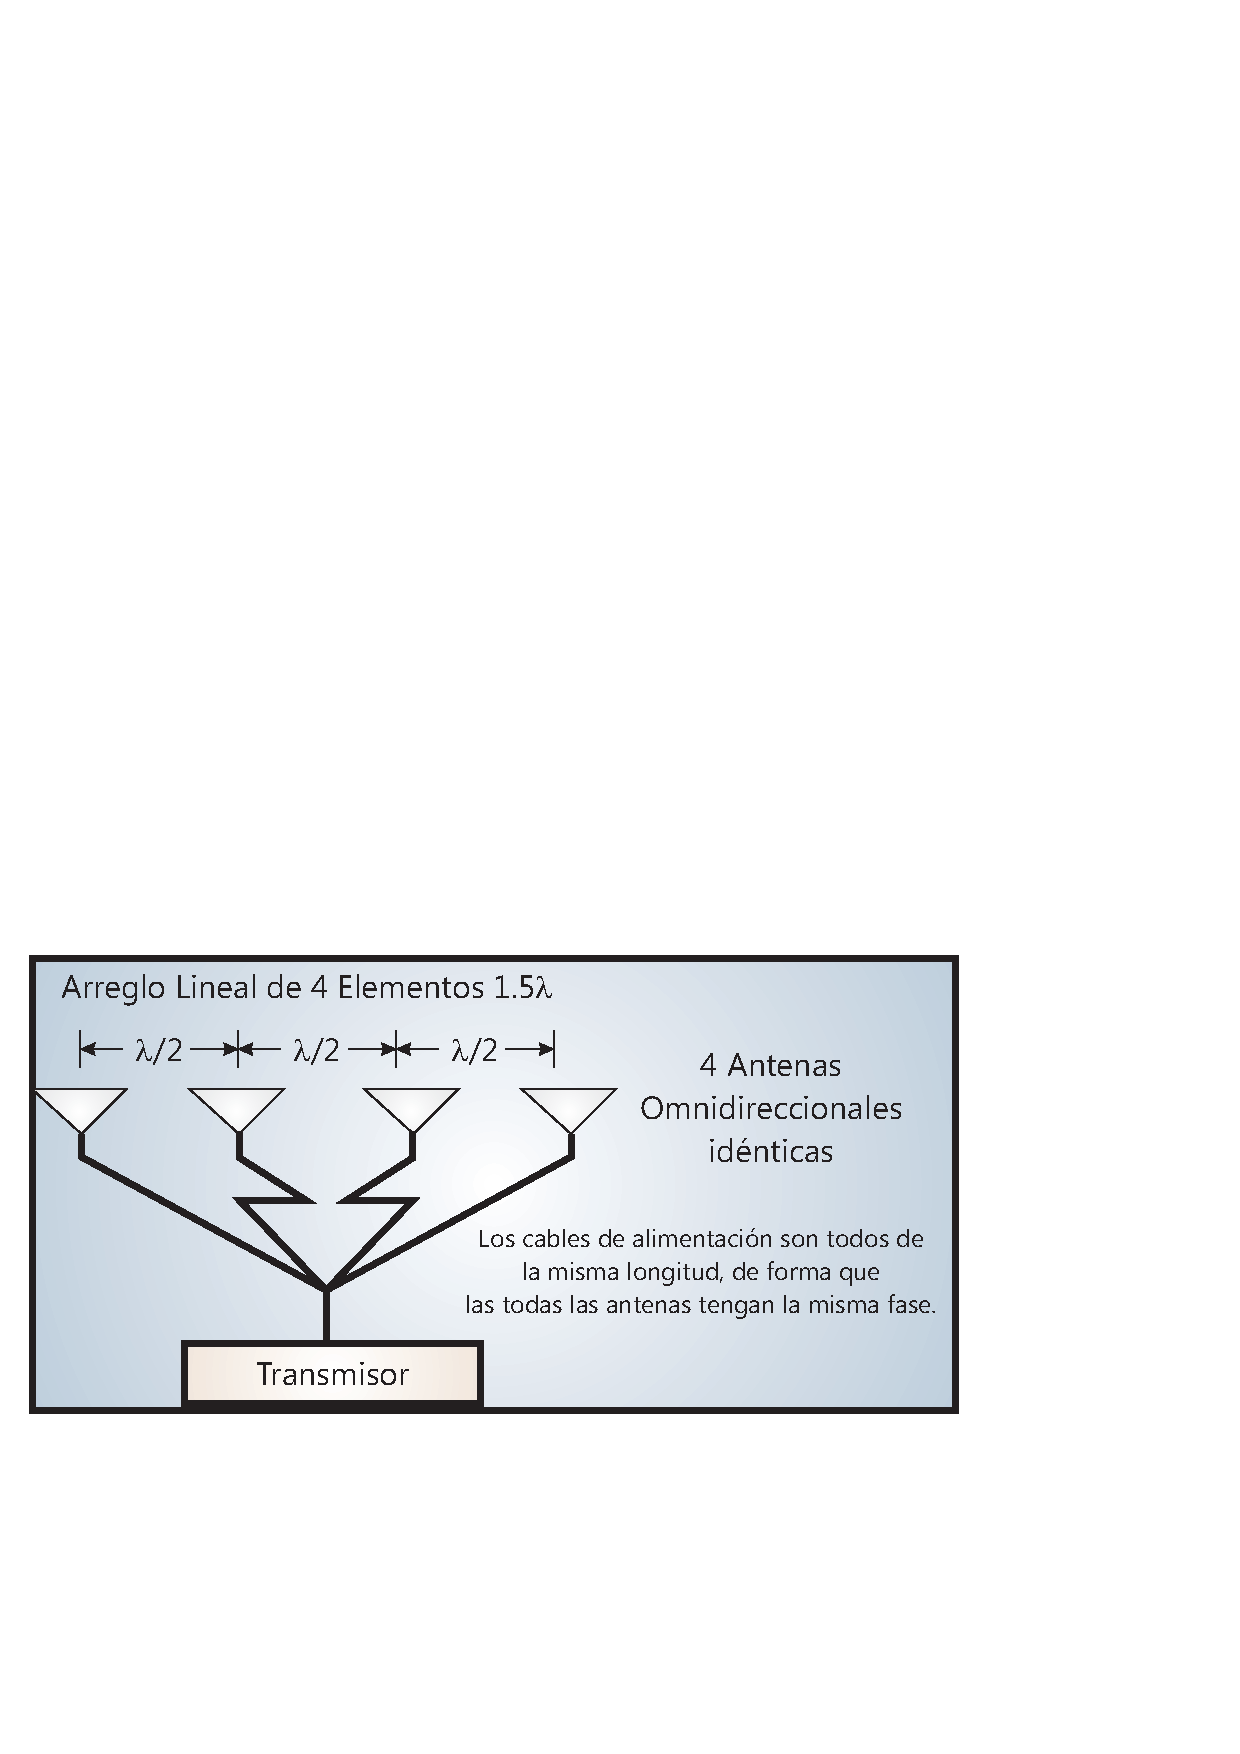
\includegraphics[width=9cm]{./figures/C02-linear_array_1_b}
        \caption{Arreglo Lineal $D=\lambda/2$ - Esquema}
        \label{fig:linear_array_1_b}
\end{figure}

Si el espaciado es incrementado a más de $1/2$ longitud de onda, empiezan a aparecer lóbulos laterales más largos en el patrón de radiación. De todas formas, el haz central se vuelve más angosto debido a que la longitud total de la antena es incrementada. A continuación se ilustra el siguiente patrón de radiación, para 4 elementos espaciados $1$ longitud de onda:

\begin{figure}[htb!]
        \centering
        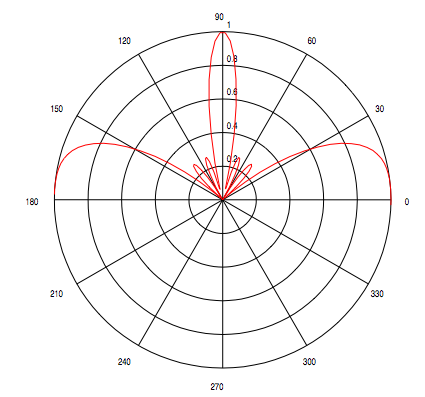
\includegraphics[width=6cm]{./figures/C02-linear_array_2}
        \caption{Arreglo Lineal $D=\lambda$ - Patrón de Radiación}
        \label{fig:linear_array_2}
\end{figure}

Al mantener la longitud total de la antena igual, y agregar elementos para reducir el espaciado nuevamente a $1/2$ longitud de onda, los lóbulos laterales se reducen. A continuación se muestra el patrón de radiación si se agregan 3 elementos más a la antena anterior para reducir el espaciado entre elementos.

\begin{figure}[htb!]
        \centering
        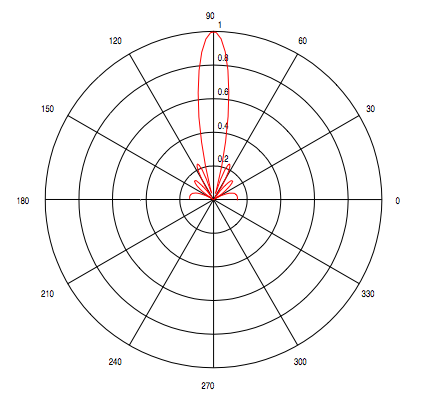
\includegraphics[width=6cm]{./figures/C02-linear_array_3}
        \caption{Arreglo Lineal $D=\lambda/2$ - 7 elementos - Patrón de Radiación}
        \label{fig:linear_array_3}
\end{figure}

\begin{figure}[htb!]
        \centering
        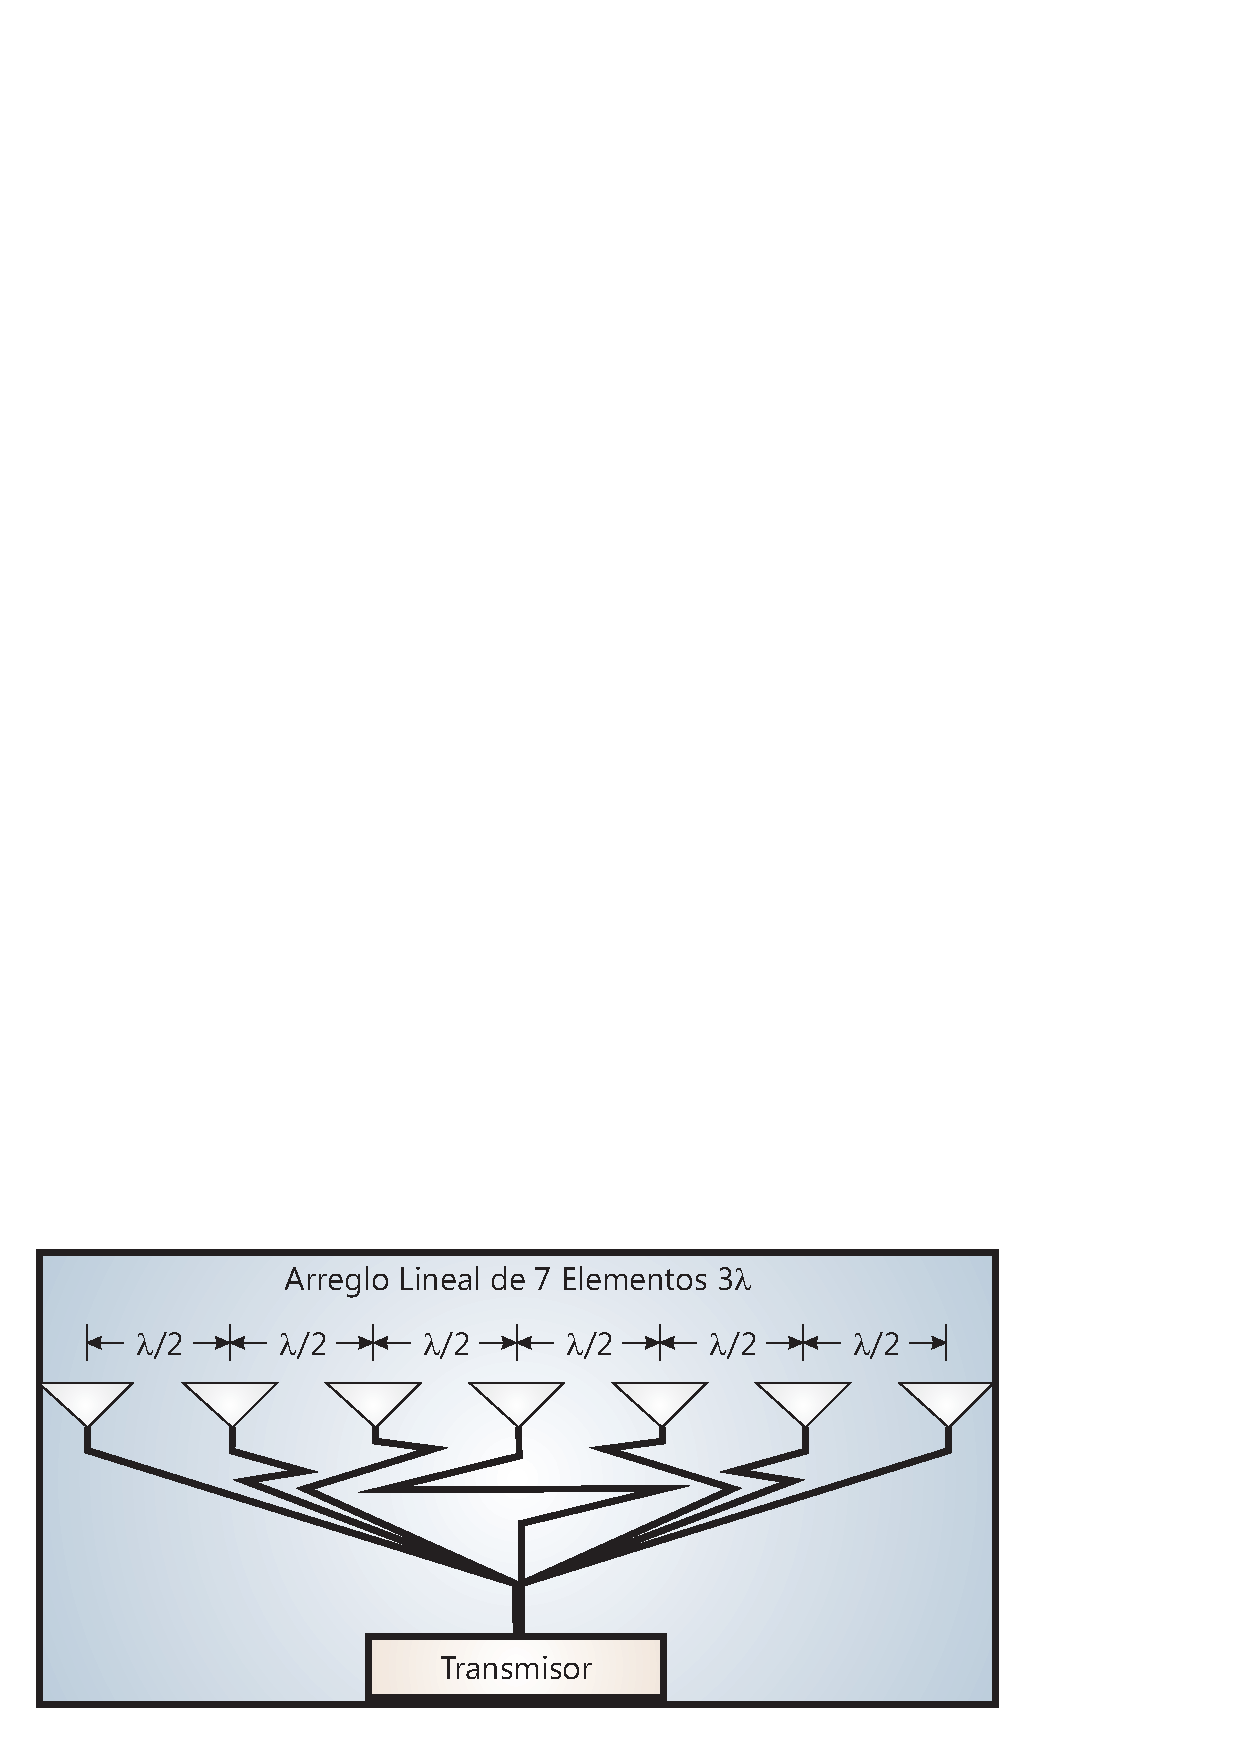
\includegraphics[width=10cm]{./figures/C02-linear_array_4}
        \caption{Arreglo Lineal $D=\lambda/2$ - 7 elementos - Esquema}
        \label{fig:linear_array_4}
\end{figure}

\subsection{Arreglos dirigidos electrónicamente}

El haz central del arreglo lineal puede ser direccionado al variar las fases de las señales en los elementos del mismo. La forma más simple para controlar la fase de las señales es variar sistemáticamente las longitudes de los cables hacia los elementos. El cable retrasa la señal, por lo cual desplaza la fase. De todas formas, esto no permite que la antena sea dirigida dinámicamente.

En un arreglo electrónicamente dirigido, se utilizan desplazadores de fase electrónicos programados en cada elemento del arreglo. La antena es dirigida al programar el valor de desplazamiento de fase requerido para cada elemento. El patrón del haz a continuación es para un arreglo lineal de 8 elementos con un desplazamiento de fase progresivo de $0,7 \pi$ por elemento. El haz central fue dirigido 45 grados a la izquierda. Un desplazamiento de fase de $2 \pi$ corresponde a una longitud de onda o un periodo de onda de portadora, y valores más positivos son equivalentes a decir que la señal es transmitida más tempranamente.

\begin{figure}[htb!]
        \centering
        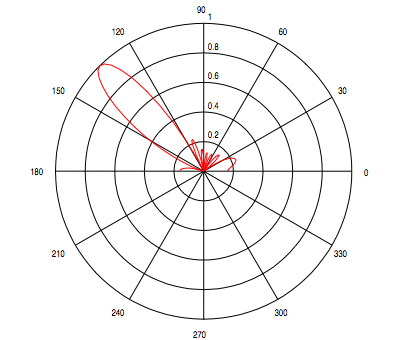
\includegraphics[width=6cm]{./figures/C02-steered_array}
        \caption{Arreglo dirigido electrónicamente - Patrón de Radiación}
        \label{fig:steered_array}
\end{figure}

\begin{figure}[htb!]
        \centering
        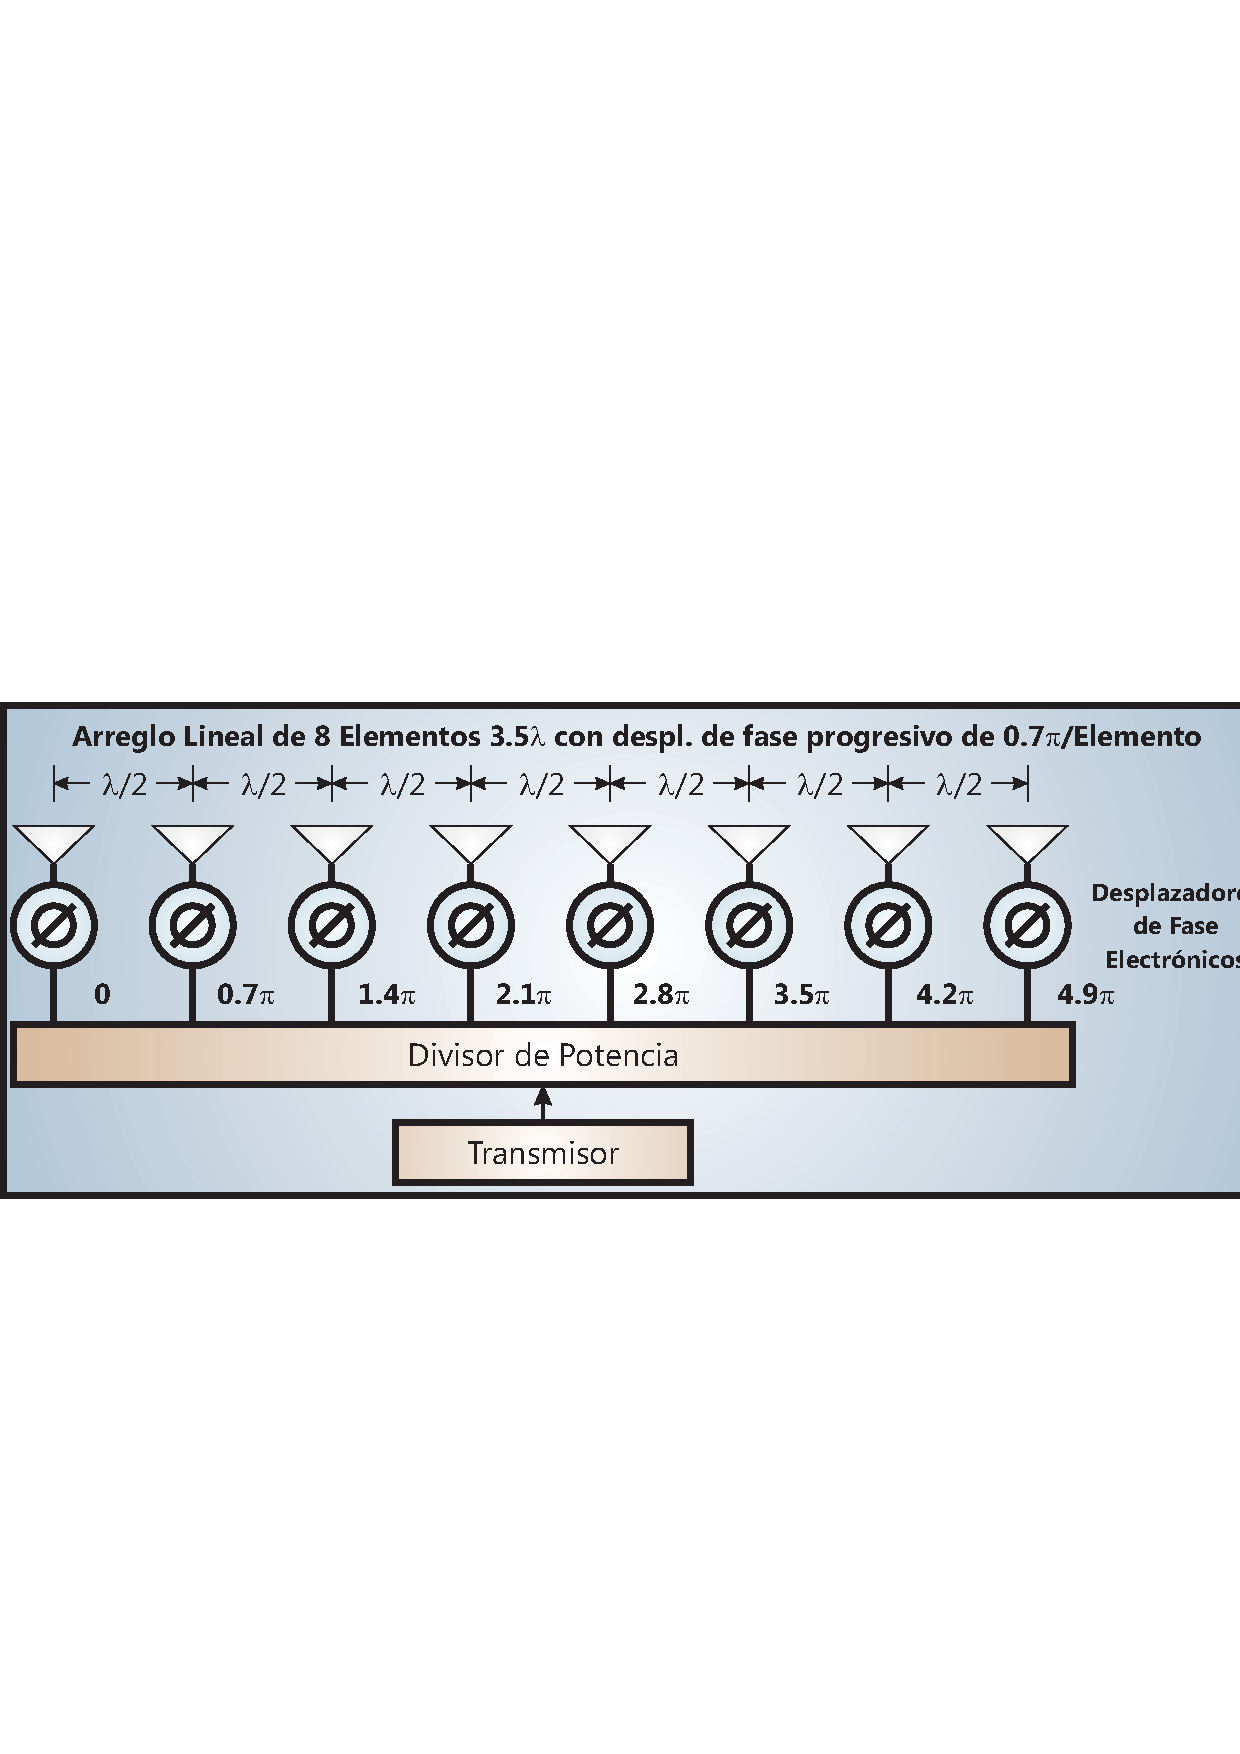
\includegraphics[width=11cm]{./figures/C02-steered_array_2}
        \caption{Arreglo dirigido electrónicamente - Esquema}
        \label{fig:steered_array2}
\end{figure}

\subsection{Parámetros básicos de arreglos de antenas}

A continuación se explicarán algunos parámetros y definiciones básicas que serán de interés relevante para los conceptos tratados en la presente tesis \cite{Litva}. A pesar de que varios de ellos son definidos en términos de antenas transmisoras, la reciprocidad asegura que estas definiciones sean también aplicables a antenas receptoras.

\subsubsection{Patrón de radiación}

Se refiere a la distribución relativa de potencia irradiada como función de la dirección en el espacio.

\subsubsection{Factor del arreglo}

El factor del arreglo representa el patrón de raciación a campo lejano de un arreglo isotrópico de elementos radiantes. El factor del arreglo se denotará a lo largo de la tesis como $F(\phi,\theta)$, donde $\phi$ representa el ángulo de azimuth y $\theta$ representa el ángulo de elevación en el espacio.

\subsubsection{Lóbulo principal}

El lóbulo principal de un patrón de radiación de una antena es el lóbulo que contiene la dirección de máxima radiación de potencia.

\subsubsection{Lóbulos laterales}

Los lóbulos laterales son lóbulos en cualquier dirección distinta de aquella del lóbulo principal. Para un arreglo lineal con ponderación uniforme, el primer lóbulo lateral (el cual es el más cercano al lóbulo principal) en el patrón de radiación se encuentra $13 dB$ por debajo del valor pico del lóbulo principal.

\subsubsection{Ancho del haz (Beamwidth)}

El ancho del haz de una antena es el ancho angular del lobulo principal en su patrón de radiación a campo lejano. El HPBW (Ancho del haz a mitad de potencia), o ancho del haz a $-3 dB$, es el ancho del haz medido entre los puntos del lóbulo principal que se encuentran a $-3 dB$ del valor pico del lóbulo principal:

\begin{equation}
HPBW = \frac{0.88 \lambda}{A}
\end{equation}

Donde $A$ representa la longitud de la apertura del arreglo.

\subsubsection{Eficiencia de la antena}

La eficiencia de la antena se define como la relación entre la potencia total irradiada por la antena y la potencia total de entrada de la misma.

\subsubsection{Ganancia directiva}

La ganancia directiva es una cantidad definida para campo lejano como la relación entre la densidad de radiación en una dirección angular particular en el espacio y la densidad de radiación de la misma potencia irradiada isotrópicamente, lo que es:

\begin{equation}
D(\phi,\theta) = \frac{4 \pi \text{ potencia irradiada por unidad de ángulo sólido en dirección } \phi,\theta }{\text{Total de potencia irradiada por la antena}}
\end{equation}

\subsubsection{Directividad}

La directividad es la máxima ganancia directiva de la antena, es decir, la ganancia directiva en la dirección de máxima densidad de radiación.

\subsubsection{Ganancia de la antena}

La ganancia de la antena es definida como la relación entre la densidad de radiación en una dirección particular del espacio y la potencia total de entrada de la antena:

\begin{equation}
G(\phi,\theta) = \frac{4 \pi \text{ potencia irradiada por unidad de ángulo sólido en dirección } \phi,\theta }{\text{Total de potencia irradiada por la antena}}
\end{equation}

La ganancia máxima G, o simplemente ganancia, es el producto entre la directividad y la eficiencia de la antena, es decir:

\begin{equation}
G = D \eta
\end{equation}

\section{\textit{Multipath fading}}

Cuando se transmite una señal a través de una antena, la misma se propaga en el medio y enfrenta distintos tipos de obstáculos, tales como el suelo, edificios, autos, personas e incluso las distintas capas de la atmósfera. Se producirán reflexiones y desfasajes que darán lugar a señales que provienen de distintos caminos o direcciones, las cuales se sumarán para obtener una señal resultante en la antena receptora. A este efecto se lo conoce como \textbf{\textit{Multipath Fading}} \cite{Pahlavan}.

\begin{figure}[htb!]
        \centering
        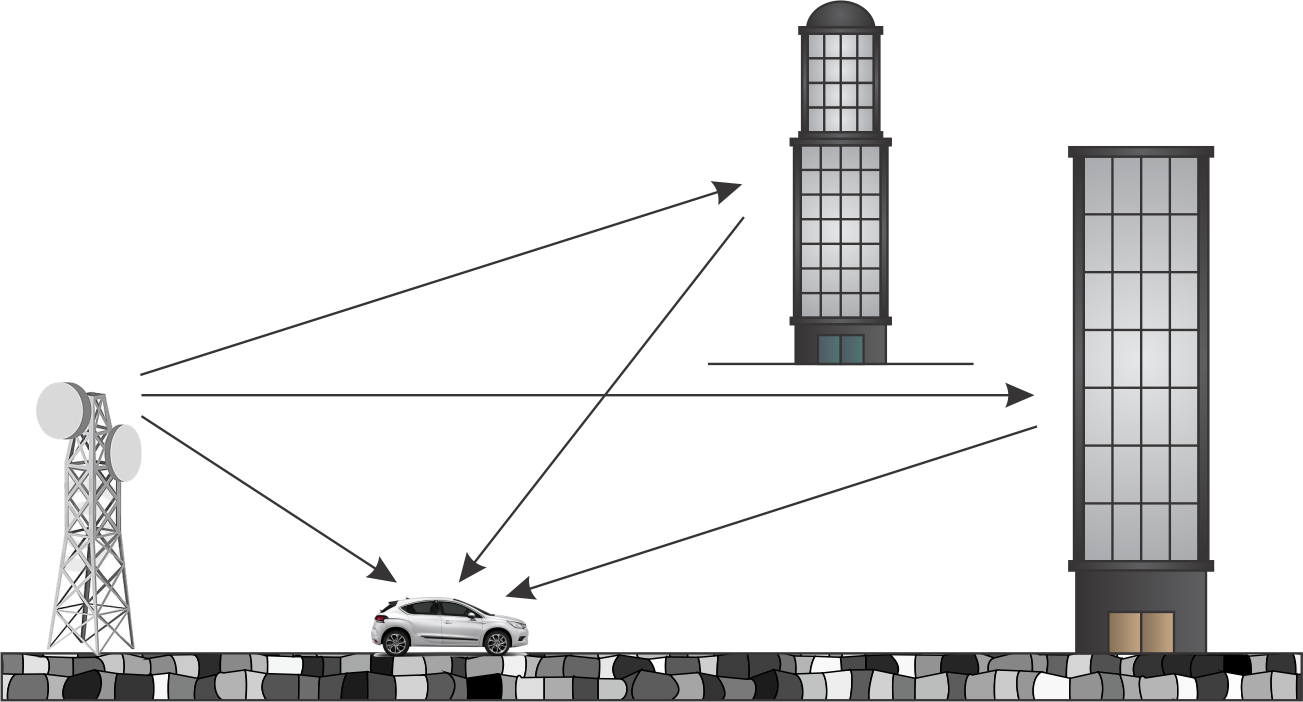
\includegraphics[width=10cm]{./figures/C02-multipath_fading}
        \caption{Múltiples Reflexiones de la señal transmitida}
        \label{fig:MultipathFading}
\end{figure}

La presencia de reflectores en el ambiente que rodea al transmisor y receptor, crea múltiples caminos que la señal transmitida puede recorrer. La amplitud y la fase de la señal que llega desde cada camino estará relacionada con la longitud del camino y las condiciones, lo cual resulta en fluctuaciones considerables en la amplitud de la señal compuesta recibida. Esto puede resultar en una interferencia constructiva o destructiva, amplificando o atenuando la potencia de señal vista desde el receptor.

El análisis preciso de la propagación por múltiples caminos puede ser abordado a través del uso de las ecuaciones de Maxwell con condiciones de contorno que representen las propiedades físicas de la arquitectura y el medio ambiente. De todas formas, este análisis es muy complejo y se suele abordar el problema haciendo una derivación a las leyes de óptica geométrica, representando a la propagación de ondas electromagnéticas como la propagación de ondas ópticas.

Cuando se produce una interferencia destructiva de gran intensidad, se la reconoce como \textbf{\textit{deep fade}} y puede resultar en una falla temporal de la comunicación debido a una severa caída en la relación señal ruido del canal.

Por dichos motivos, es deseable encontrar una forma de poder abordar el fenómeno de \textit{multipath fading} con el objetivo de poder garantizar estabilidad y confiabilidad en la comunicación.

\section{\textit{Beamforming}}

\textit{Beamforming} consiste en la combinación de distinas señales de radio provenientes de un conjunto de antenas no direccionales, espacialmente separadas, con el objetivo de simular una gran antena direccional \cite{Haynes}. La antena simulada puede ser apuntada electrónicamente, a pesar de que físicamente, la antena no se mueva. En comunicaciones, la técnica de \textit{beamforming} es utilizada para apuntar una antena hacia la fuente de la señal para reducir la interferencia y mejorar la calidad de la comunicación. En aplicaciones de descubrimiento de dirección, \textit{beamforming} puede ser utilizado para dirigir una antena para determinar la dirección del origen de una señal.

\subsection{\textit{Beamforming} digital}

La técnica de \textit{beamforming} digital está basada en la conversión de una señal de RF proveniente de cada antena a dos flujos de señales binarias en banda base representando los canales I y Q \cite{Litva}. Las señales digitales en banda base luego representan las amplitudes y fases de las señales recibidas en cada elemento del arreglo. El proceso de \textit{beamforming} implica la ponderación de estas señales digitales, ajustando sus amplitudes y fases de forma tal que al ser sumadas en conjunto formen el haz deseado. Básicamente, un sistema de \textit{beamforming} digital consta de un arreglo de antenas, receptores individuales para cada una de ellas, y un procesador digital de señales.

\begin{figure}[htb!]
        \centering
        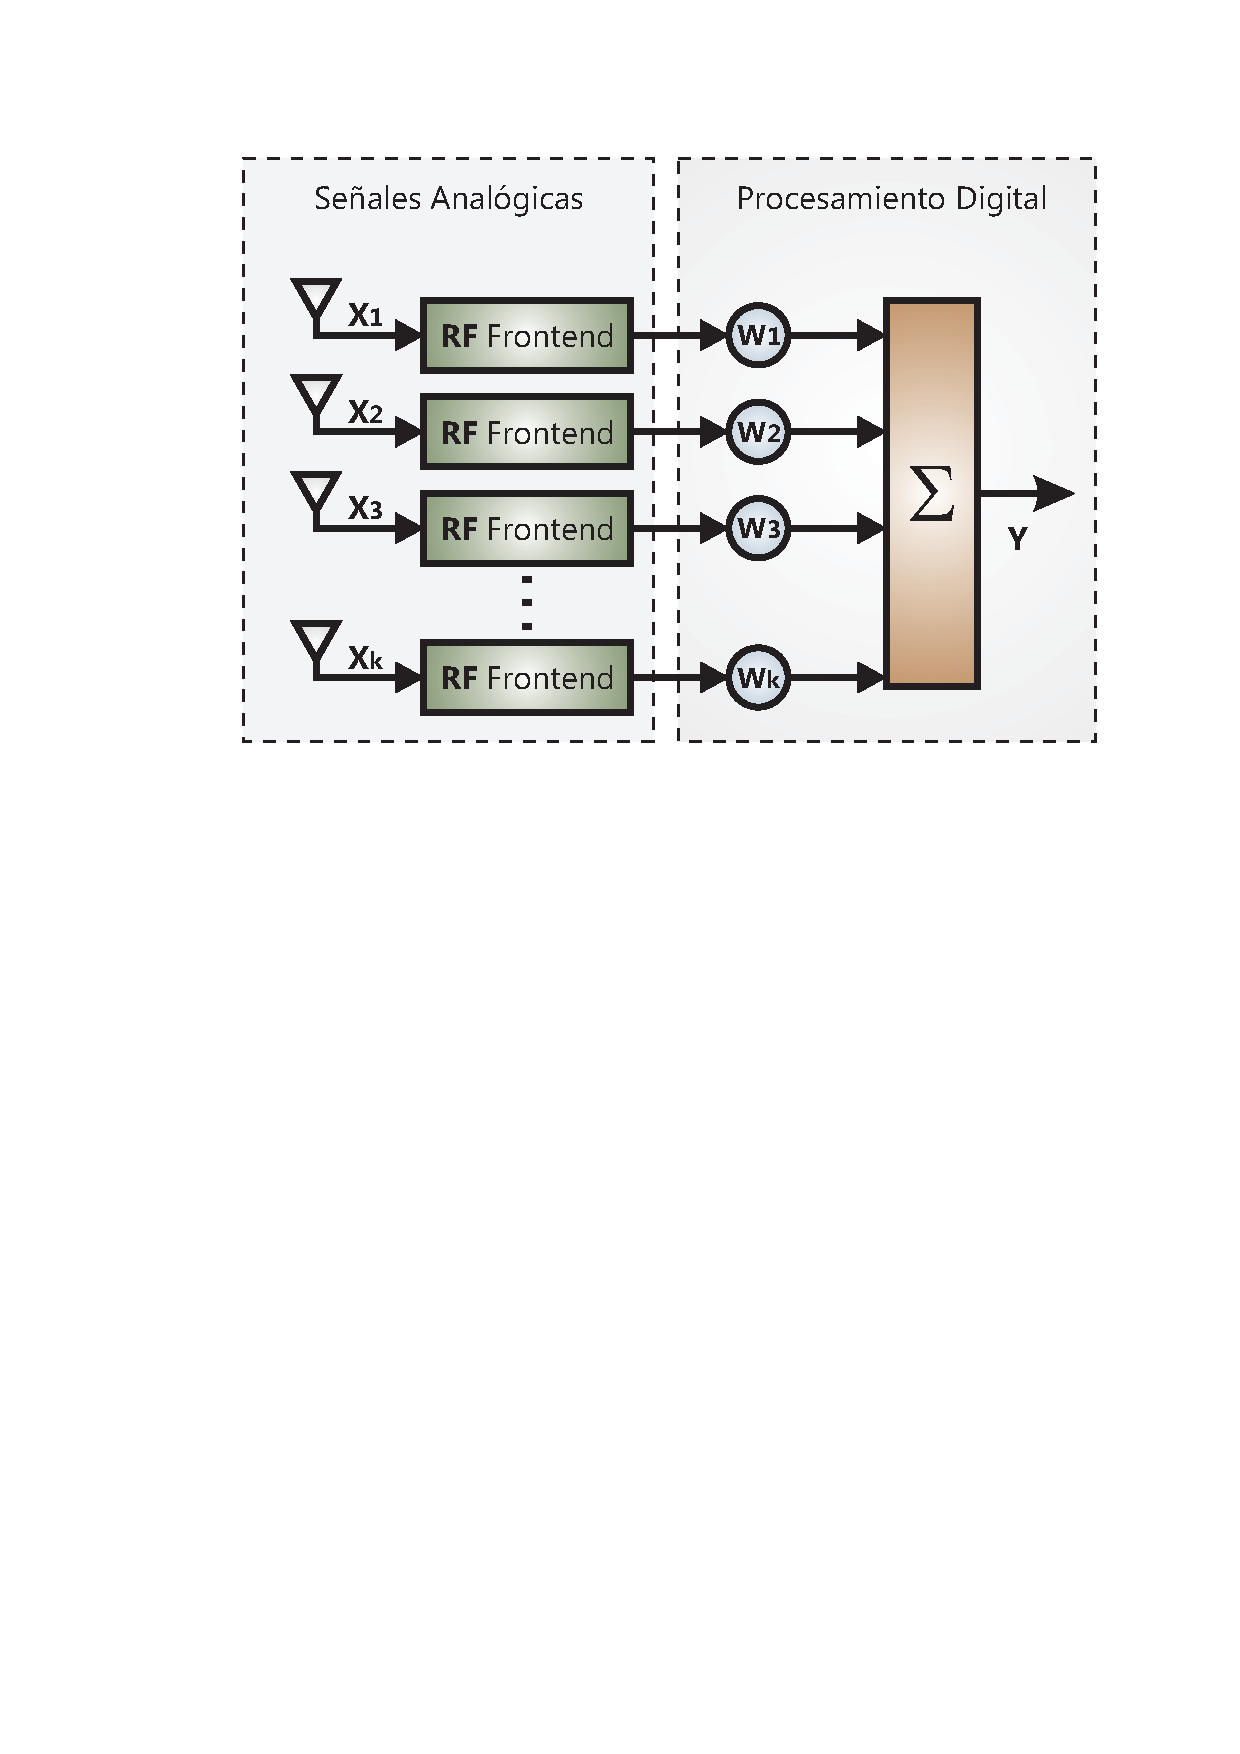
\includegraphics[width=10cm]{./figures/C02-beamforming}
        \caption{Esquema de un sistema de \textit{Beamforming}}
        \label{fig:Beamforming}
\end{figure}

Se puede observar en la \textbf{figura \ref{fig:Beamforming}} que las señales provenientes de cada una de las antenas son registradas por un frontend de RF en el cual se considera que está presente toda la circuitería analógica requerida para adaptar la señal y el conversor A/D utilizado para transformarla a un stream digital. Las señales digitales obtenidas ingresan luego al procesador digital en el cual se implementan los pesajes $w_1, w_2, ..., w_k$ para obtener una suma ponderada de las mismas.

Tanto la amplitud como la fase de cada antena pueden ser controladas. La combinación del control de fase y amplitud puede ser utilizada para ajustar los lóbulos laterales y dirigir nulos mejor que lo que se puede lograr con el control de fase por si solo. La amplitud relativa $a_k$ y desplazamiento de fase $\theta_k$ para cada antena es llamado un ``peso complejo'' y es representado por una constante compleja $w_k$ (para la antena en la $k^{\text{ésima}}$ posición)

Un \textit{beamformer} para un transmisor de radio aplica los coeficientes de ponderación a la señal a transmitir (desplaza la fase y aplica la amplitud) para cada elemento del arreglo de antenas.

Un \textit{beamformer} para la recepción en radio aplica los pesos complejos a la señal de cada antena, y luego suma todas las señales para formar aquella que tiene el patrón direccional deseado.

Las primeras ideas que formaron las bases del \textit{beamforming} digital fueron desarrolladas por investigadores en las áreas de sistemas de radar y sonar. El \textit{beamforming} digital es una unión entre las tecnologías de antena y las tecnologías digitales. Una antena puede ser considerada un dispositivo que convierte señales espacio-temporales en señales estrictamente temporales, haciéndolas disponibles a una gran variedad de técnicas de procesamiento de señales. De esta forma, toda la información deseada que está siendo transportada por estas señales puede ser extraída.

Una ventaja mayor del \textit{beamforming} digital radica en el hecho de que una vez que la información de RF es capturada en la forma de un flujo digital, dicho contenido está disponible para la aplicación de una gran cantidad de técnicas de procesamiento digital de señales. 

El haz deseado es formado en el dominio digital (dentro del sistema de procesamiento). Para diseñar el sistema de procesamiento pueden utilizarse distintas tencologías, tales como FPGA, DSPs de propósito general o chips específicamente diseñados para \textit{beamforming}. El procesamiento digital requiere que la señal de cada antena sea digitalizada utilizando un conversor A/D. Debido a que las señales de radio por encima de las frecuencías de onda corta ($>30 MHz$) son muy altas para ser digitalizadas directamente a un costo razonable, los receptores de \textit{beamforming} digital utilizan ``traductores de RF'' para desplazar la frecuencia de la señal hacia niveles inferiores antes de los conversores A/D. La clave de esta tecnología es lograr una traducción precisa de la señal analógica al régimen digital. Esto se logra utilizando receptores heterodinos completos, los cuales deben estar cercanamente apareados en amplitud y fase. Los receptores deben realizar el pasaje a frecuencias inferiores, filtrado y amplificación a un nivel de potencia adaptado a los requerimientos de entrada de los conversores A/D.


\subsection{\textit{Beamforming} adaptativo}

Un \textit{beamformer} adaptativo es un dispositivo que tiene la capacidad de separar señales en el dominio del espacio. Este hecho provee un medio para separar la señal deseada de señales de interferencia. Un \textit{beamformer} adaptativo logra optimizar automaticamente el patrón del arreglo al ajustar el control de los pesos de ponderación hasta que se satisface una determinada función de objetivo prestablecida. Los medios por los cuales esta optimización es lograda están especificados por un algoritmo diseñado para tal propósito. Estos dispositivos utilizan mucha más información disponible en la antena con respecto a un \textit{beamformer} convencional.

\begin{figure}[htb!]
        \centering
        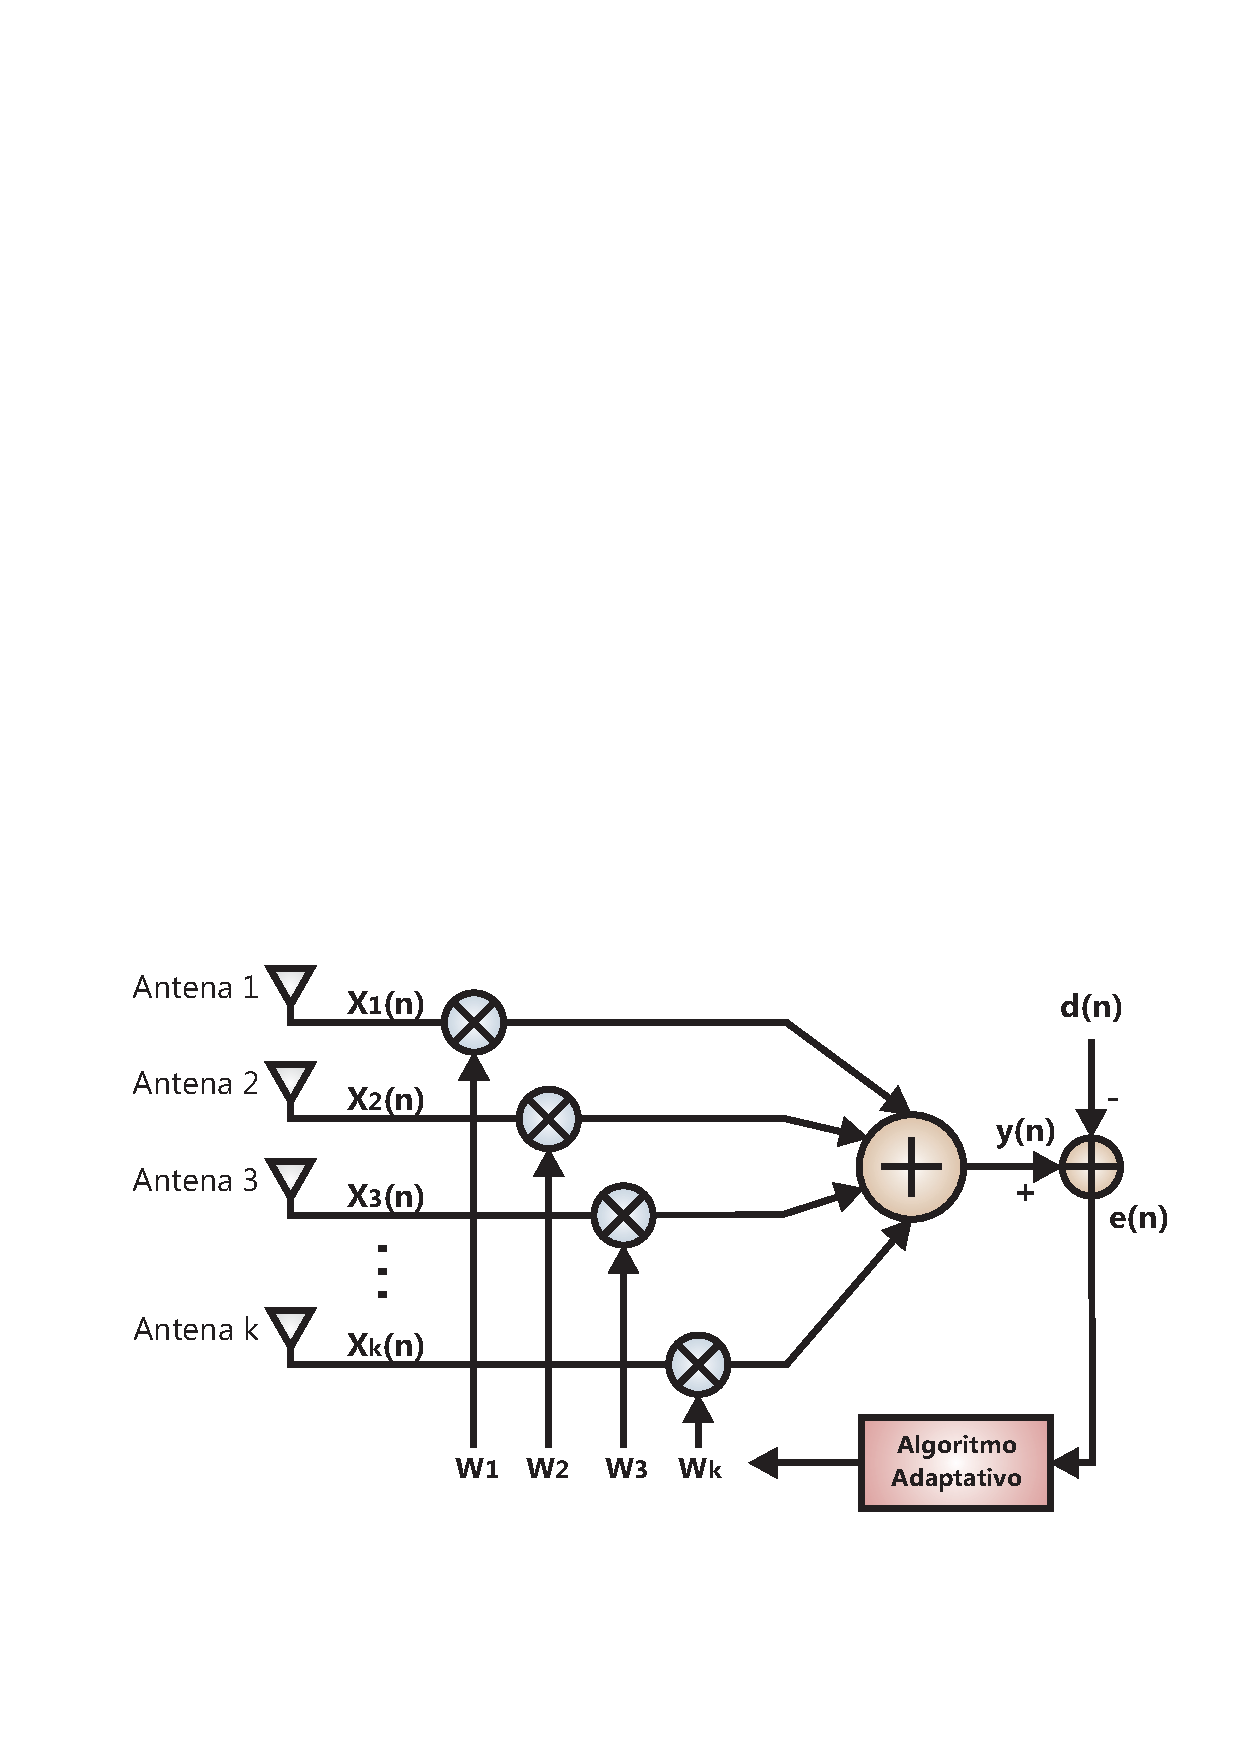
\includegraphics[width=10cm]{./figures/C02-adaptive_beamforming}
        \caption{Esquema de un sistema de \textit{Beamforming} Adaptativo}
        \label{fig:Adaptive_Beamforming}
\end{figure}

\subsubsection{Conceptos básicos}

El procedimiento utilizado para direccionar y modificar el patrón del haz del arreglo con el objetivo de mejorar la recepción de la señal deseada, mientras simultáneamente se suprimen las señales de interferencia a través de la seleción de pesos complejos, se puede exponer como se explica a continuación.

Se tiene un arreglo como el expuesto en la figura \ref{fig:example}, que consiste de dos antenas omnidireccionales con espaciado $\lambda_0/2$. La señal deseada, $S(t)$ llega desde la dirección de máxima ganancia ($\Theta_S = 0$), y la señal de interferencia, $I(t)$ llega desde el ángulo ($\Theta_1 = \pi / 6$).

\begin{figure}[htb!]
        \centering
        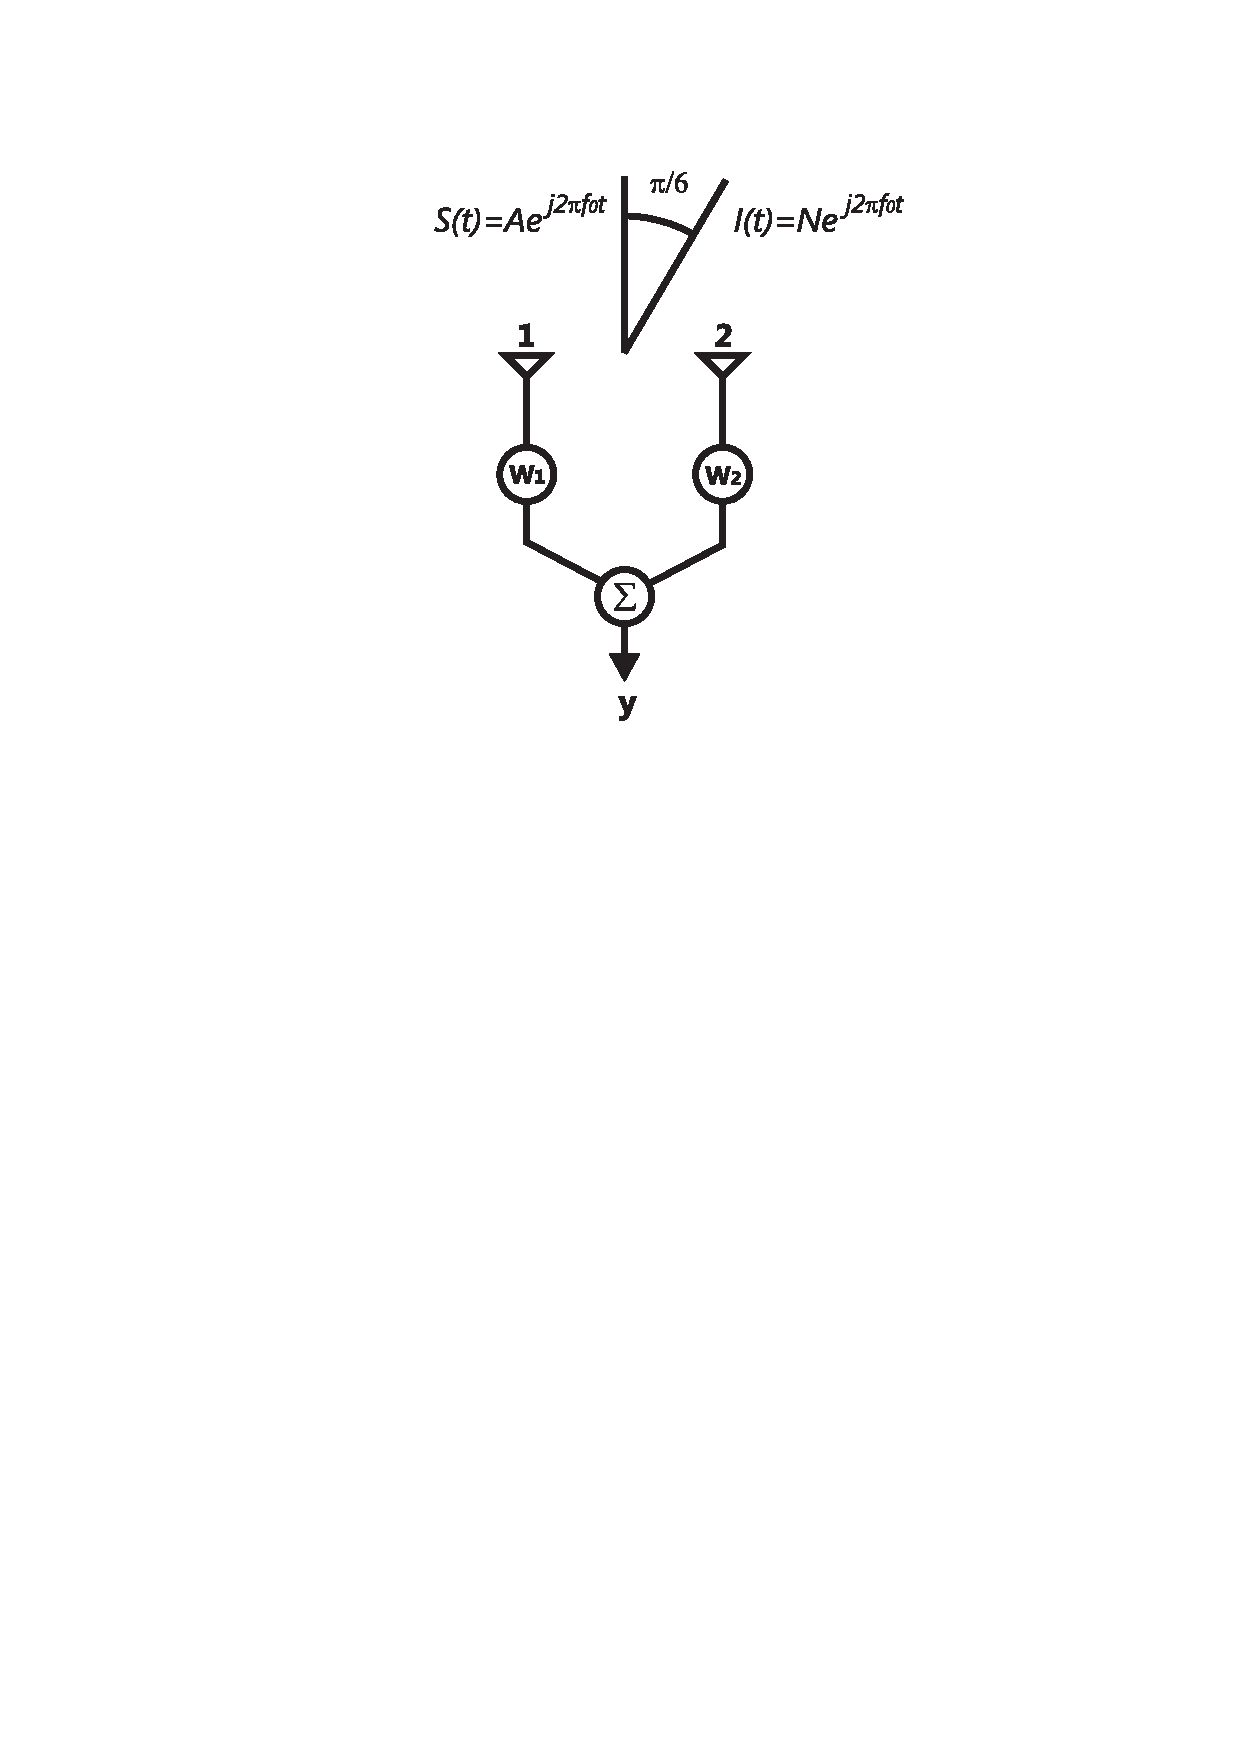
\includegraphics[width=7cm]{./figures/C02-example}
        \caption{Arreglo de dos elementos para la supresión de interferencia}
        \label{fig:example}
\end{figure}

Ambas señales tienen la misma frecuencia $f_o$. La señal de cada antena es multiplicada por una variable de ponderación compleja, y las señales ponderadas son luego sumadas para formar la salida del arreglo. La contribución de señal deseada en la salida del arreglo es:

\begin{equation}
y_d(t) = A e^{j 2 \pi f_o t}(w_1 + w_2)
\end{equation}

Para que $y_d(t)$ sea igual a S(t), es necesario que

\begin{equation}
\begin{array}{l}
\Re[w_1] + \Re[w_2] = 1\\
\Im[w_1] + \Im[w_2] = 0 \label{desired_condition1}
\end{array}
\end{equation}

Donde $\Re[]$ e $\Im[]$ corresponden a las componentes real e imaginaria respectivamente. La señal de interferencia incidente llega al elemento 2 con una dirección de fase con respecto al elemento 1 de valor $2 \pi \frac{1}{\lambda_0} d sin (\pi / 6) = \pi / 2$. Consecuentemente, la contribución de señal de interferencia en la salida del arreglo es:

\begin{equation}
y_i(t) = N e^{j 2 \pi f_o t}w_1 + N e^{(j 2 \pi f_o t + \pi / 2)} w_2 
\end{equation}

Para que la respuesta de interferencia del arreglo sea cero es necesario que

\begin{equation}
\begin{array}{l}
\Re[w_1] + \Re[jw_2] = 0\\
\Im[w_1] + \Im[jw_2] = 0 \label{desired_condition2}
\end{array}
\end{equation}

La solución simultánea para las ecuaciones \eqref{desired_condition1} y \eqref{desired_condition2} lleva a:

\[
w_1 = \frac{1}{2} - j \frac{1}{2} \hspace{3cm} w_2 = \frac{1}{2} + j \frac{1}{2}
\]

Con estos pesos, el arreglo aceptará la señal deseada mientras que simultáneamente rechazará la interferencia.

El ejemplo expuesto toma ventaja en el hecho de que sólo hay un único origen de interferencia direccional y que utiliza la información a priori sobre la frecuencia y dirección de ambas señales. Un procesador práctico no debería requerir ese nivel de detalles en la información a priori sobre la ubicación, número y naturaleza de las fuentes de señal.

De todas formas, el ejemplo muestra que un sistema compuesto por un arreglo, que es configurado con pesos complejos, provee posibilidades innumerables para realizar los objetivos del sistema. Sólo se necesita desarrollar un procesador adaptativo práctico para llevar a cabo el ajuste en los pesos complejos.

\subsection{Criterios para obtener los pesos óptimos}

A continuación se mencionan algunos criterios existentes para la elección de los pesos óptimos para el filtro adaptativo. Se verá que cada uno de ellos se puede expresar como una solución a la \textbf{ecuación de Wiener Hopf}.

\subsubsection{Mínimo error cuadrático medio}

Considerar inicialmente un arreglo de antenas uniformemente espaciado, el cual opera en un ambiente de señal donde se tiene una señal de comunicación desada $s(t)$, así como tambien $N_u$ señales de interferencia $\{u_i(t)\}^{N_u}_{i=1}$. Luego considerar que las señales deseadas llegan al arreglo con un ángulo espacial $\theta_0$ y que la señal de interferencia $i$ llega con un ángulo $\theta_i$. La salida del arreglo es representada por:

\begin{equation}
\mathbf{x}(t) = s(t) \mathbf{v} + \mathbf{u} = \mathbf{s} + \mathbf{u}
\end{equation}

$\mathbf{v}$ consiste en el vector de propagación del arreglo para la señal deseada:

\begin{equation}
\mathbf{v}^T = [1,e^{j k d sin \theta_0} ... e^{j k (K-1) d sin \theta_0}]
\end{equation}

$\mathbf{u}$ representa la suma de todos los vectores de señales de interferencia:

\begin{equation}
\mathbf{u}^T = \sum_{i=1}^{N_u} u_i(t) \boldsymbol\eta_i
\end{equation}

y $\boldsymbol\eta_i$ es el vector de propagación del arreglo para la $i^{\text{ésima}}$ señal de interferencia.

\begin{equation}
\boldsymbol\eta_i^T = [1, e^{j k d sin \theta_i} ... e^{j k (K-1) d sin \theta_i}]
\end{equation}

Si la señal deseada $s(t)$ es conocida, uno puede elegir minimizar el error entre la salida del \textit{beamformer} $\mathbf{w}^H \mathbf{x}(t)$ y la señal deseada. Por supuesto, el conocimiento de la señal deseada eliminiaría la necesidad del \textit{beamformer}. De todas formas, para muchas aplicaciones, las características de la señal deseada pueden ser conocidas con suficiente detalle para generar una señal $d^*(t)$ que la representa cercanamente, o que por lo menos se correlaciona con la señala deseada en un cierto nivel. Esta señal es llamada la \textbf{señal de referencia}. Se expresa a la señal de referencia como un complejo conjugado sólo por conveniencia matemática. Los pesos son elegidos para minimizar el error cuadrático medio (MSE) entre la salida del \textit{beamformer} y la señal de referencia:

\begin{equation}
\epsilon^2(t) = [d^*(t) - \mathbf{w}^H \mathbf{x}(t)]^2
\label{mse}
\end{equation}

Al tomar la esperanza en ambos lados de la ecuación \eqref{mse} y llevar a cabo algunas manipulaciones algebráicas, se tiene:

\begin{equation}
E\{\epsilon^2(t)\} = E\{d^*(t)\} - 2 \mathbf{w}^H \mathbf{r} + \mathbf{w}^H \mathbf{R} \mathbf{w}
\label{mse_E}
\end{equation}

donde $\mathbf{r} = E\{d^*(t)x(t)\}$ y $\mathbf{R} = E\{\mathbf{x}(t)\mathbf{x}^H(t)\}$. $\mathbf{R}$ es usualmente referida como la matriz de covarianza. El mínimo error cuadrático medio se obtiene al igualar a cero el gradiente del vector de la ecuación \eqref{mse_E} con respecto a $\mathbf{w}$.

\begin{equation}
\nabla \mathbf{w} (E\{ \epsilon^2(t)\}) = -2 \mathbf{r} + 2 \mathbf{R} \mathbf{w} = 0
\label{nabla_to_zero}
\end{equation}

La solución a esta ecuación es

\begin{equation}
\mathbf{w}_{opt} = \mathbf{R}^{-1} \mathbf{r}
\label{wiener}
\end{equation}

la cual es referida como la ecuación de Wiener-Hopf o la solución óptima Wiener. Si $s(t) = d^*(t)$ luego $\mathbf{r} = E\{d^2(t)\} \mathbf{v}$. Se puede expresar $\mathbf{R} = E\{d^2(t)\} \mathbf{v v^H} + \mathbf{R}_u$, donde $\mathbf{R}_u = E\{\mathbf{u u^H}\}$ y aplicar la \textit{Identidad de Woodbury} a $\mathbf{R^{-1}}$ y se tiene:

\begin{equation}
\mathbf{R^{-1}} = \Bigg[ \frac{1}{1 + E\{d^2(t)\} \mathbf{v^H R_u^{-1} v}} \Bigg] \mathbf{R_u^{-1}}
\end{equation}

Luego, la solución de Wiener se puede generalizar como:

\begin{equation}
\mathbf{w}_{\text{opt}} = \beta \mathbf{R_u^{-1}v}
\end{equation}

Donde $\beta$ es el coeficiente escalar. En el caso del mínimo MSE:

\begin{equation}
\beta = \frac{E\{d^2(t)\}}{1 + E\{d^2(t)\} \mathbf{v^H R_u^{-1} v}}
\end{equation}

\subsubsection{Máxima relación señal interferencia}

Los pesos pueden ser elegidos para maximizar la relación señal interferencia (SIR). Si se asume que $\mathbf{R_s} = E\{\mathbf{s s^H}\}$ y $\mathbf{R_u} = E\{\mathbf{u u^H}\}$ son conocidas, se puede elegir maximizar la relación de la potencia de señal de salida $\sigma_s^2$ y el total de potencial de señal de interferencia $\sigma_u^2$. La potencia de señal de salida puede expresarse como:

\begin{equation}
\sigma_s^2 = E\{|\mathbf{w^H s}|^2\} = \mathbf{w^H R_s w}
\end{equation}

y la potencia de salida de ruido como:

\begin{equation}
\sigma_u^2 = E\{|\mathbf{w^H u}|^2\} = \mathbf{w^H R_u w}
\end{equation}

Luego, la SIR está dada por:

\begin{equation}
\text{SIR} = \frac{\sigma_s^2}{\sigma_u^2} = \frac{\mathbf{w^H R_s w}}{\mathbf{w^H R_u w}}
\label{SIR}
\end{equation}

Tomando la derivada de (\ref{SIR}) con respecto a $\mathbf{w}$ e igualándola a cero se obtiene:

\begin{equation}
\mathbf{R_s w} = \frac{\mathbf{w^H R_s w}}{\mathbf{w^H R_u w}} \mathbf{R_u w}
\end{equation}

lo cual consiste en un problema de autovalores. El valor de $\frac{\mathbf{w^H R_s w}}{\mathbf{w^H R_u w}}$ está delimitado por los autovalores mínimo y máximo de la matriz simétrica $\mathbf{R_u^{-1} R_s}$. El máximo autovalor $\lambda_{\text{max}}$ que satisface

\begin{equation}
\mathbf{R_u^{-1} R_s w} = \lambda_{\text{max}} \mathbf{w}
\end{equation}

es el óptimo valor de SIR. Correspondiente a este valor, existe un único autovector, $w_{\text{opt}}$ que representa a los pesos óptimos. Luego:

\begin{equation}
\mathbf{R_s w_{\text{opt}}} = \text{SIR} \hspace{1mm} \mathbf{R_u w_{\text{opt}}}
\end{equation}

Notando que $\mathbf{R_s} = E\{d^2(t)\} \mathbf{v v^H}$, se obtiene:

\begin{equation}
\mathbf{w}_{\text{opt}} = \beta \mathbf{R_u^{-1}v}
\end{equation}

donde

\begin{equation}
\beta = \frac{E\{d^2(t)\}}{\text{SIR}} \mathbf{v^H w_\text{opt}}
\end{equation}

Lo cual representa que el criterio del máximo SIR puede ser también expresado en términos de la solución de Wiener.

\subsubsection{Varianza mínima}

Si la señal deseada y su dirección son desconocidas, una forma de asegurar una buena recepción de señal es minimizar la varianza del ruido de salida. Recordando que la salida del \textit{beamformer} es:

\begin{align}
y(t) &=  \mathbf{w^H x} \\
     &=  \mathbf{w^H s + w^H u} \nonumber
\end{align}

Para asegurar que la señal deseada es enviada con una ganancia y fase específica, se puede utilizar una restricción de forma que la respuesta del \textit{beamformer} para la señal deseada sea:

\begin{equation}
\mathbf{w^H v} = g
\label{constraint}
\end{equation}

La minimización de las contribuciones a la salida a causa de la interferencia es lograda a través de la elección de los pesos para minimizar la varianza de la potencia de salida

\begin{align}
\text{Var}\{y\} &=  \mathbf{w^H R w} \\
                &=  \mathbf{w^H R_s w + w^H R_u w} \nonumber 
\end{align}

sujeta a la restricción definida en (\ref{constraint}). Esto es equivalente a minimizar la cantidad $\mathbf{w^H R_u w}$. Utilizando el método de Lagrange, se tiene

\begin{equation}
\mathbf{\nabla w}\Bigg(\frac{1}{2} \mathbf{w^H R_u w} + \beta [1 - \mathbf{w^H v}]\Bigg) = \mathbf{R_u w} - \beta \mathbf{v}
\end{equation}

de forma tal que

\begin{equation}
\mathbf{w}_\text{opt} = \beta \mathbf{R_u^{-1} v}
\label{variance_solution}
\end{equation}

donde

\begin{equation}
 \beta = \frac{g}{\mathbf{v^H R_u^{-1} v}}
\end{equation}

La solución \ref{variance_solution} es también una solución de Wiener. Si $g = 1$, la respuesta del \textit{beamformer} es normalmente conocida como la respuesta de mínima varianza sin distorción (MVDR).

\section{Algoritmos adaptativos}

En la sección anterior, se mostró que los criterios óptimos estan íntimamente relacionados entre si. Por lo cual, la elección del criterio no es crítica en términos de rendimiento.

Por otro lado, la elección de \textbf{algoritmos adaptativos} para derivar los pesos adaptativos es muy importante, dado que determina tanto la velocidad de convergencia como la complejidad de hardware requerida para implementar el algoritmo. A continuación se discutiran algunas de las técnicas adaptativas más comunes.

\subsection{Algoritmo LMS - \textit{Least Mean Squares}}

El algoritmo adaptativo más común para adaptatividad continua es el \textbf{algoritmo LMS}. Se basa en el método de descenso más pronunciado, que computa y actualiza recursivamente el vector de pesos. Es razonablemente intuitivo que correcciones sucesivas al vector de pesos en la dirección negativa del vector gradiente deberían eventualmente llevar al MSE, hasta un punto tal que el vector de pesos asume su valor óptimo. De acuerdo al método, el valor actualizado del vector de pesos en el momento $n + 1$ es computado utilizando la siguiente relación recursiva simple

\begin{equation}
\mathbf{w}(n + 1) \approx \mathbf{w}(n) + \frac{1}{2} \mu [-\mathbf{\nabla}(E\{\epsilon^2(n)\})]
\end{equation}

Reemplazando con (\ref{nabla_to_zero}) se obtiene

\begin{equation}
\mathbf{w}(n + 1) = \mathbf{w}(n) + \mu [\mathbf{r} - \mathbf{R w}(n)]
\end{equation}

En la realidad, una medición exacta del vector gradiente no es posible, dado que esto requeriría un conocimiento previo tanto de $\mathbf{R}$ como de $\mathbf{r}$. La estrategia más obvia consiste en usar estimaciones instantáneas, las cuales son definidas respectivamente como:

\begin{equation}
\mathbf{\hat{R}}(n) = \mathbf{x}(n) \mathbf{x}^H(n)
\end{equation}

y

\begin{equation}
\mathbf{\hat{r}}(n) = \hat{d}(n) \mathbf{x}(n)
\end{equation}

Los pesos pueden ser actualizados como

\begin{align}
\mathbf{\hat{w}}(n + 1) &= \mathbf{\hat{w}}(n) + \mu \mathbf{x}(n)[\hat{d}(n) - \mathbf{x}^H(n)\mathbf{\hat{w}}(n)] \\
                        &= \mathbf{\hat{w}}(n) + \mu \mathbf{x}(n) \hat{e}(n) \nonumber 
\end{align}

La constante de ganancia $\mu$ controla las características de convergencia del vector de secuencia aleatorio $\mathbf{w}(n)$. Se debe notar que este es un enfoque continuamente adaptativo, en el cual los pesos son actualizados a medida que los datos son muestreados de forma tal que el vector resultante converja a la solución óptima. La adaptatividad continua funciona bien cuando las estadísticas relacionadas con el ambiente de la señal son \textbf{estacionarias}. La figura \ref{fig:lms_algorithm} muestra la representación gráfica del flujo de la señal del \textbf{algoritmo LMS}. La virtud principal de este algoritmo es su simplicidad. El rendimiento es aceptable en diversas aplicaciones. De todas formas, sus características de convergencia dependen en la estructura de autovalores de $\mathbf{\hat{R}}$. Cuando éstos están ampliamente difundidos, la convergencia puede ser lenta y debería considerarse utilizar otros algoritmos adaptativos con tasas de convergencia más altas.

\begin{figure}[htb!]
        \centering
        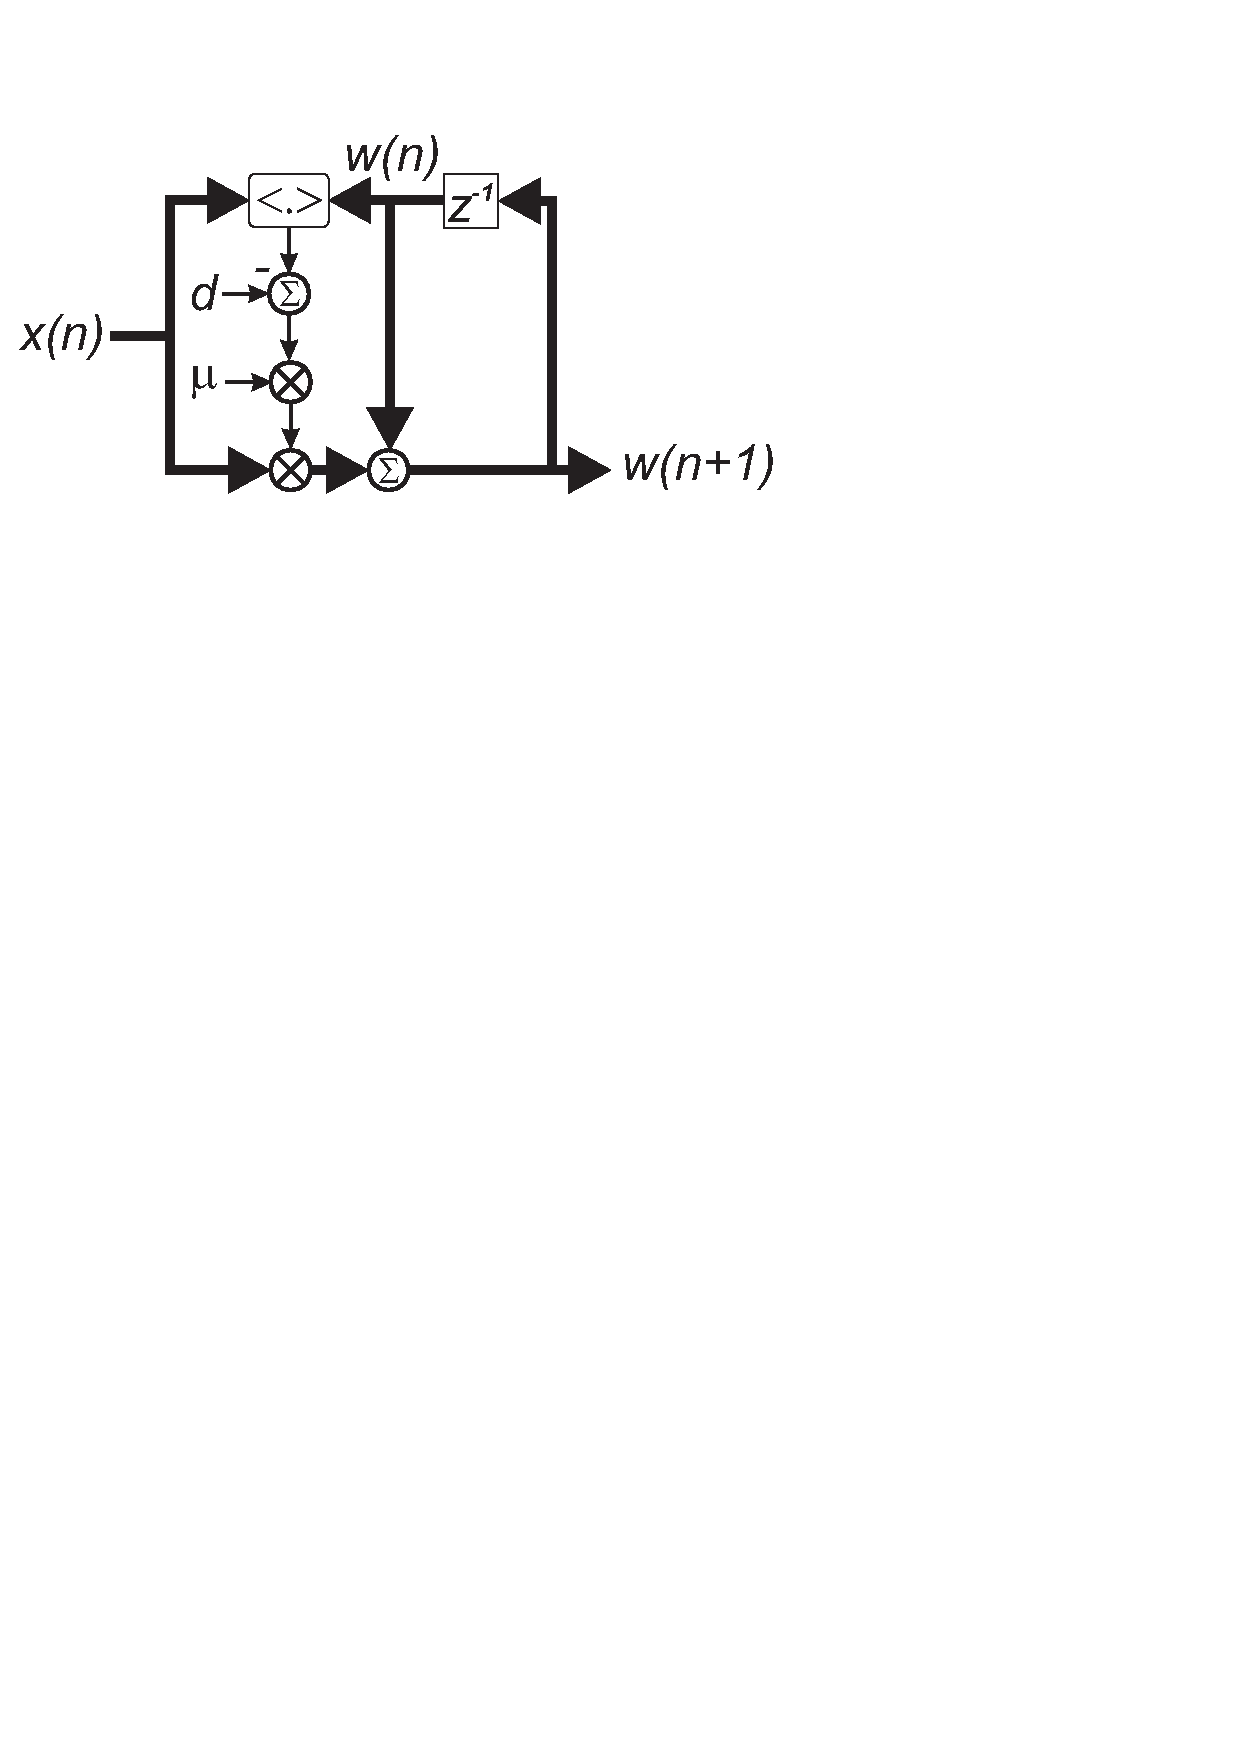
\includegraphics[width=6cm]{./figures/C02-lms_signal_flow}
        \caption{Representación gráfica del flujo de señal para el algoritmo LMS}
        \label{fig:lms_algorithm}
\end{figure}

\subsection{Algoritmo RLS - \textit{Recursive Least Squares}}

En este algoritmo se realiza la estimación de $\mathbf{R}$ y $\mathbf{r}$ realizando una suma ponderada:

\begin{equation}
\mathbf{\hat{R}}(n) = \sum_{i=1}^N \gamma^{n-1} \mathbf{x}(i) \mathbf{x}^H(i)
\label{estimate_R}
\end{equation}

y

\begin{equation}
\mathbf{\hat{r}}(n) = \sum_{i=1}^N \gamma^{n-1} \hat{d}(i) \mathbf{x}(i)
\label{estimate_r}
\end{equation}

El factor de ponderación, $0 < \gamma \leq 1$ tiene la función de asegurar que los datos en el pasado son ``olvidados'' con el objetivo de permitir que el procesador siga las variaciones estadísticas de los datos observables. Factorizando los términos correspondientes a $i = n$ tanto en (\ref{estimate_R}) y (\ref{estimate_r}), se tiene la siguiente recursión para actualizar tanto $\mathbf{\hat{R}}(n)$ y $\mathbf{\hat{r}}(n)$:

\begin{equation}
\mathbf{\hat{R}}(n) = \gamma \mathbf{R}(n-1) + \mathbf{x}(i) \mathbf{x}^H(n)
\end{equation}

y

\begin{equation}
\mathbf{\hat{r}}(n) = \gamma \mathbf{\hat{r}}(n-1) + \hat{d}(n) \mathbf{x}(n)
\end{equation}

Utilizando la identidad de Woodbury, se puede obtener la siguiente ecuación recursiva para llegar a la inversa de la matriz de covarianza:

\begin{equation}
\mathbf{R}^{-1}(n) = \gamma^{-1} [\mathbf{R}^{-1}(n-1) - \mathbf{q}(n) \mathbf{x}(n) \mathbf{R}^{-1}(n-1) ] 
\end{equation}

donde el vector de ganancia $\mathbf{q}(n)$ está dado por:

\begin{equation}
\mathbf{q}(n) = \frac{\gamma^{-1} \mathbf{R}^{-1}(n-1) \mathbf{x}(n)}{1 + \gamma^{-1} \mathbf{x}^H(n) \mathbf{R}^{-1}(n-1) \mathbf{x}(n)}
\end{equation}

Para desarrollar la ecuación recursiva para actualizar el estimador de cuadrados mínimos $\mathbf{\hat{w}}(n)$ se usa (\ref{wiener}) para expresar $w(n)$ como sigue:

\begin{align}
\mathbf{\hat{w}}(n) &= \mathbf{R}^{-1}(n) \mathbf{r}(n) \\
                    &= \gamma^{-1} [ \mathbf{R}^{-1}(n-1) - \mathbf{q}(n)\mathbf{x}(n) \mathbf{R}^{-1}(n-1)] \nonumber \\
                    &\qquad \times [\gamma \mathbf{r}(n-1) + \hat{d}(n) \mathbf{x}(n)]
                    \nonumber
\end{align}

Reorganizando la ecuación, se puede actualizar el peso como sigue:

\begin{equation}
\mathbf{\hat{w}}(n) = \mathbf{\hat{w}}(n-1) + \mathbf{q}(n) [ \hat{d}(n) - \mathbf{\hat{w}}^H (n-1) \mathbf{x}(n) ]
\end{equation}

Una característica importante del algoritmo RLS es que la inversión de la matriz de covarianza $\mathbf{x}(n)$ es reemplazada en cada paso por una división escalar simple. La figura \ref{fig:rls_algorithm} muestra la representación del flujo de señal del algoritmo RLS. La tasa de convergencia para el algoritmo RLS es típicamente un orden de magnitud más alta que la del algoritmo LMS.

\begin{figure}[htb!]
        \centering
        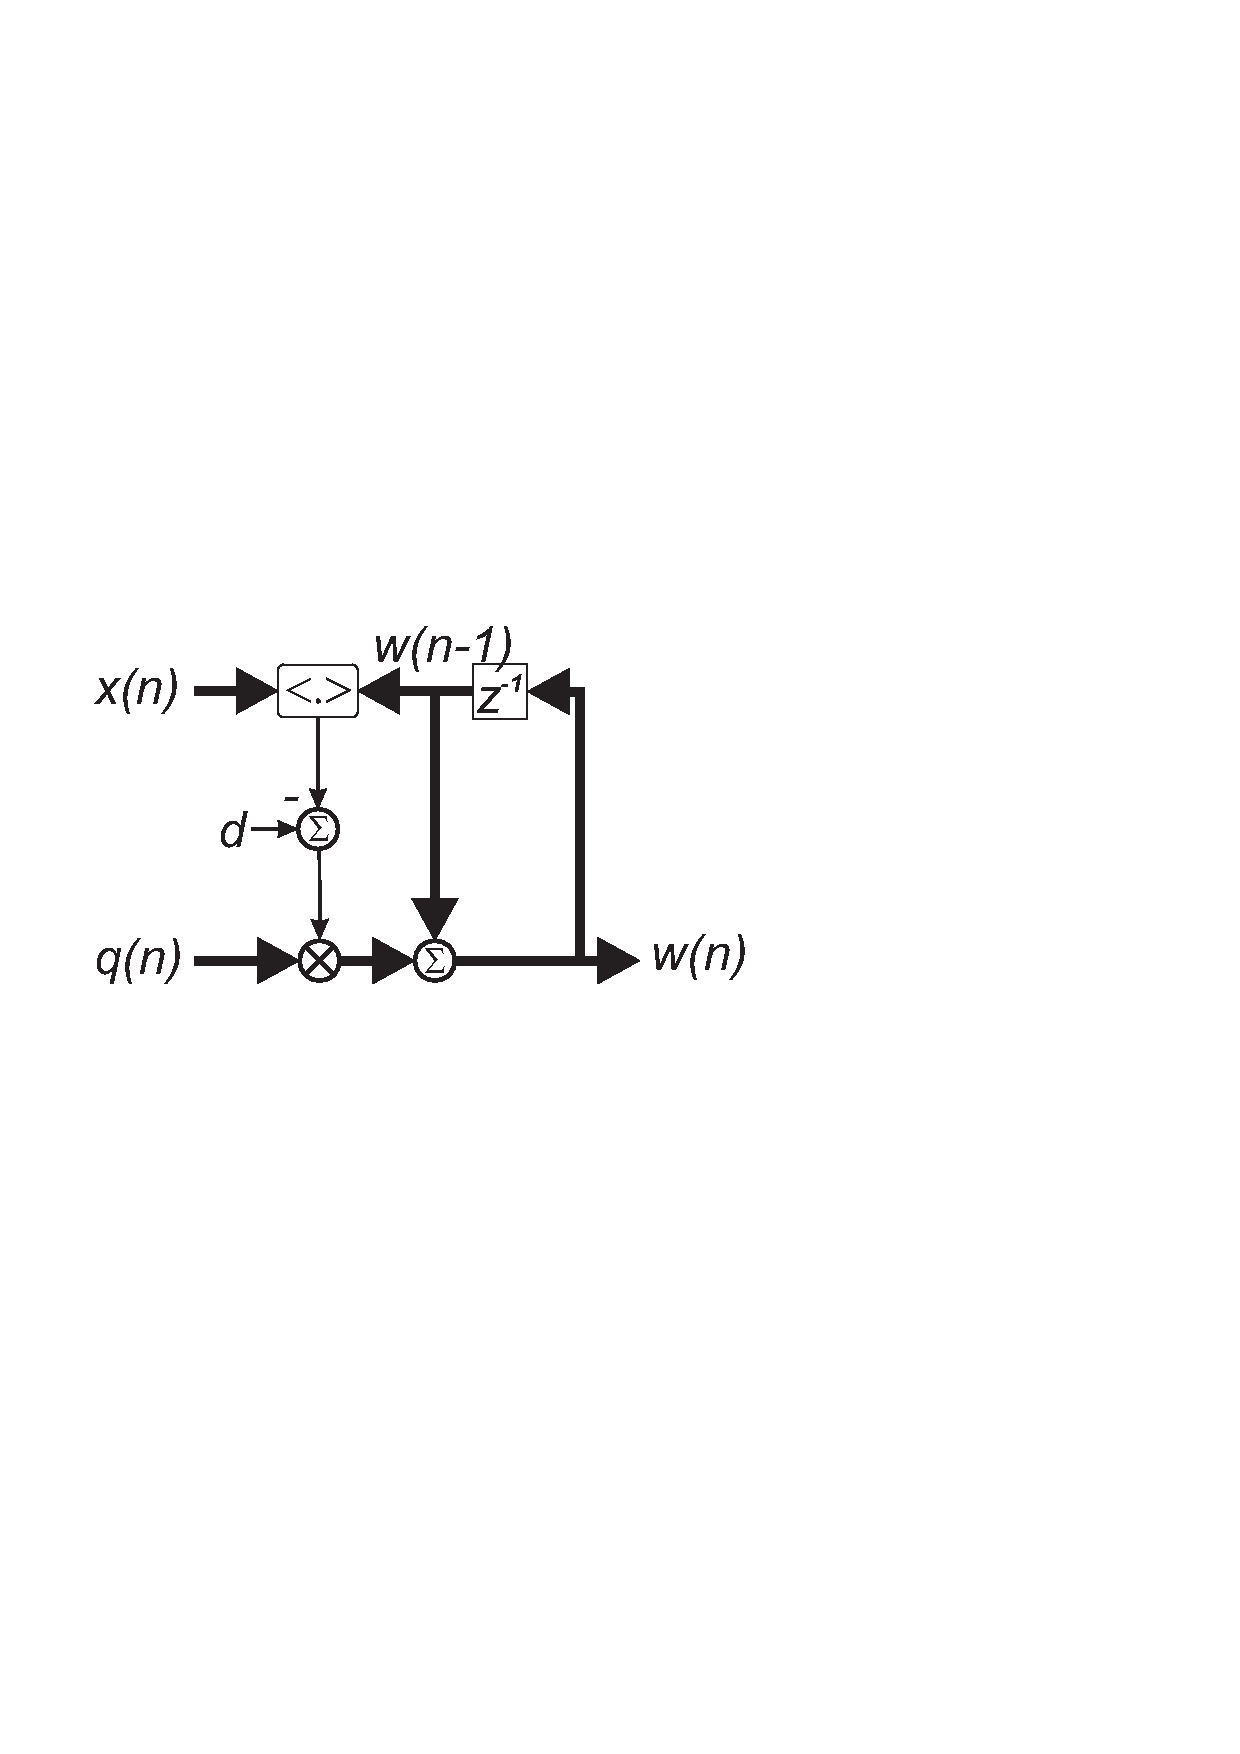
\includegraphics[width=6cm]{./figures/C02-rls_signal_flow}
        \caption{Representación gráfica del flujo de señal para el algoritmo RLS}
        \label{fig:rls_algorithm}
\end{figure}

\subsection{Adquisición de la señal de referencia}

Se han planteado distintos criterios y algoritmos para realizar \textit{beamforming} adaptativo. Todos ellos requieren algún tipo de señal de referencia en su proceso de optimización adaptativa. Cuando se habla de señales de referencia, normalmente se refiere a información a priori y explícita o conocimientos sobre las señales de interés. Una referencia explícita puede ser dividida en dos categorías: referencia espacial y referencia temporal. La primera es refereida normalmente como la información de ángulo de arribo (AOA - \textit{Angle of Arrival}) de la señal deseada. Una señal de referencia temporal puede ser una señal piloto que está correlacionada con la señal deseada, una secuencia especial incluida en un paquete por la señal deseada, o un código pseudo-ruido (PN - \textit{pseudo-noise}) conocido en un sistema CDMA. La forma de referencia disponible depende del sistema particular donde se implementará el \textit{beamforming} adaptativo. Si una señal de referencia explícita está disponible en el sistema, se la debe ustilizar tanto como sea posible para lograr menor complejidad, mayor precisión y convergencia rápida.

Es valioso describir el proceso de adquisición de la señal de referencia en un sistema CDMA. El \textit{beamforming} adaptativo es muy adecuado para un sistema CDMA, debido a que los códigos de dispersión pueden ser usados como referencias para \textit{beamforming}. La implementación común de \textit{beamforming} adaptativo en un sistema de comunicaciones wireless CDMA es el uso del lazo de generación de referencia de Compton. Una configuración de implementación genérica para \textit{beamforming} adaptativo en CDMA se muestra en la figura \ref{fig:reference_signal_flow}. En esta configuración, la demodulación es realizada luego del \textit{beamforming}. Esto es, la salida del arreglo es primero mezclada con una señal de un oscilador local codificada CDMA, la cual es filtrada y limitada. La señal limitada es re-modulada a través de una mezcla con la señal del oscilador local codificado CDMA correspondiente.  La señal remodulada es usada como señal de referencia, la cual es comparada con la salida retrasada del arreglo para producir una señal de error. La señal de error dirige al procesador adaptativo para actualizar los pesos de \textit{beamforming}. El loop de retroalimentación es no lineal debido a la operación de limitación.

\begin{figure}[htb!]
        \centering
        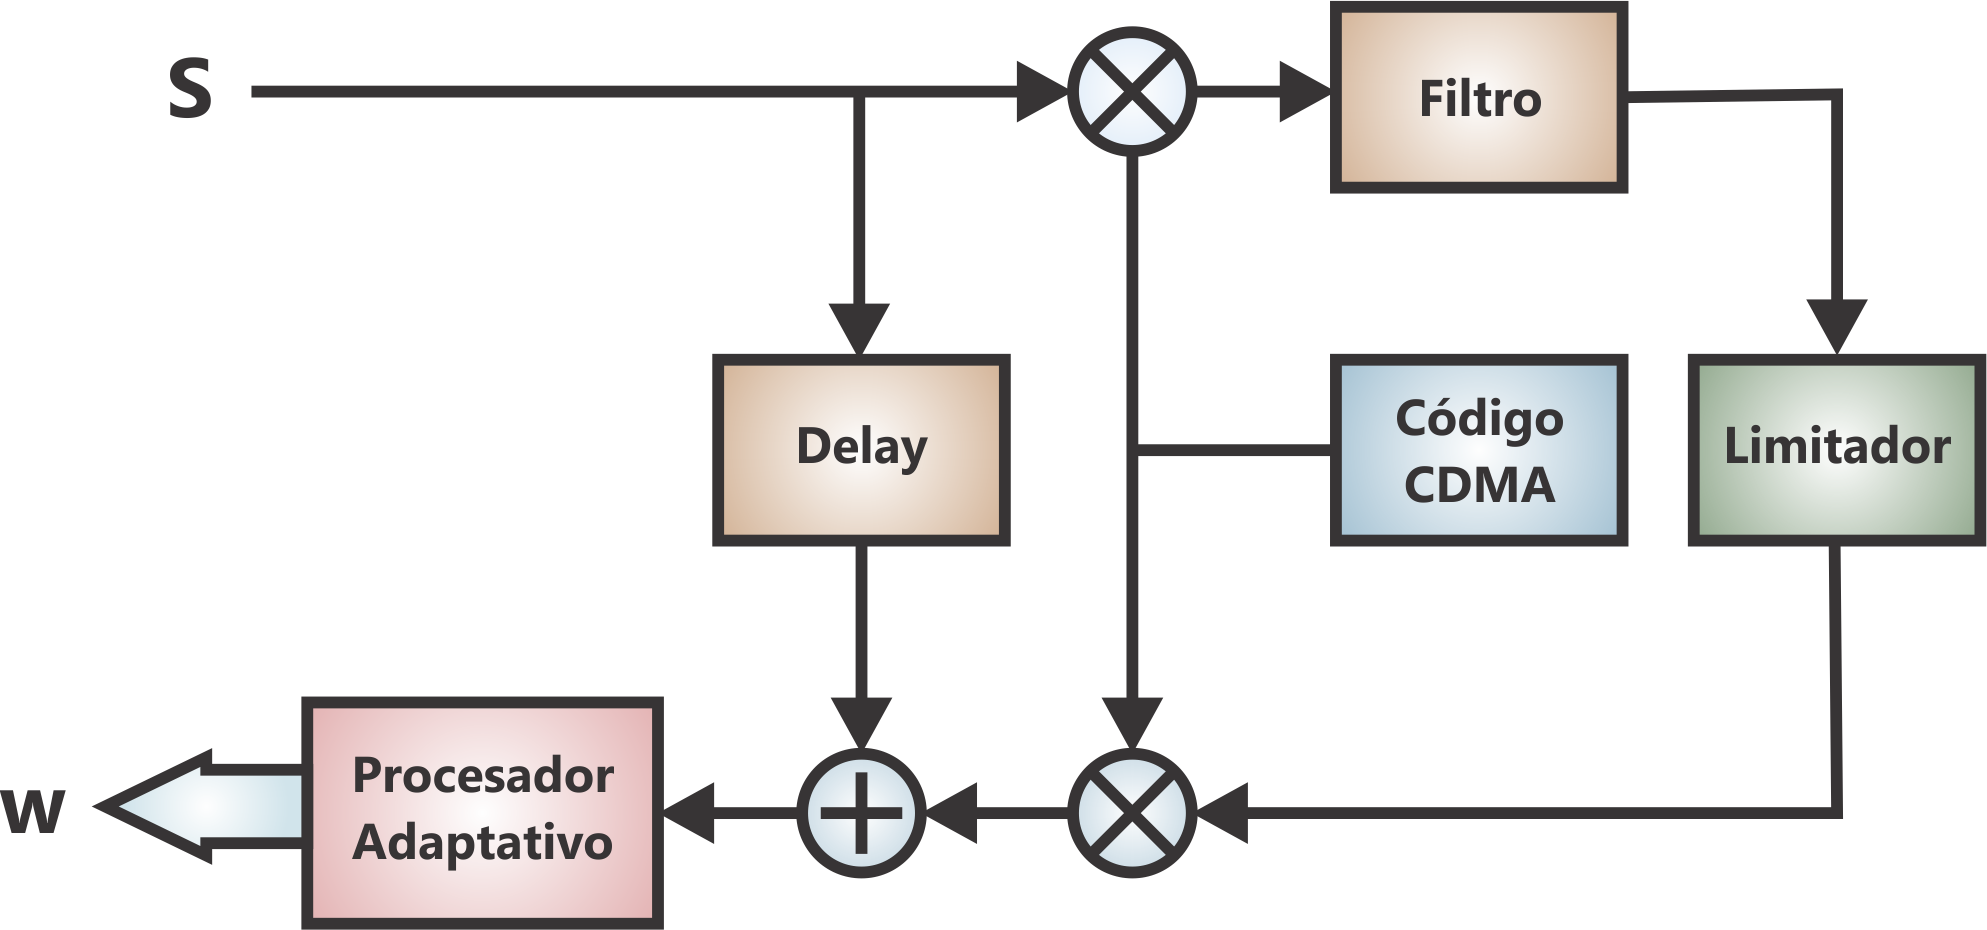
\includegraphics[width=9cm]{./figures/C02-reference_signal_flow}
        \caption{Una configuración genérica para \textit{beamforming} adaptativo en un sistema de comunicación wireless CDMA}
        \label{fig:reference_signal_flow}
\end{figure}

\section{Otras técnicas de diseño MIMO}

Los sistemas MIMO pueden ser diseñados para proveer máxima diversidad para incrementar la confiabiliad de la transmisión, o para alcanzar una máxima ganancia de multiplexado para soportar altos niveles de tasas de transmisión.

La capacidad de un canal MIMO puede ser mucho más alta que la de un sistema SISO. Este rendimiento de un sistema MIMO es cuantificado a través de la ganancia de multiplexado espacial.

Si distintas copias de la señal son transmitidas o recibidas desde múltiples antenas, los sistemas pueden mejorar la confiabilidad de un enlace inalámbrico. Esta ganancia es llamada ganancia de diversidad.

Los sistemas MIMO pueden ser utilizados simultáneamente para proveer tanto ganancia por diversidad como por multiplexado. De todas formas, existe una relación de compromiso entre ellos.

\subsection{\textit{Space-Time block coding}}

En este tipo de diseño, se toman copias de la señal, las cuales son transmitidas desde múltiples antenas o son recibidas en más de una antena en sistemas multi-antena espacio-tiempo. La probabilidad de error promedio de símbolo de un sistema de comunicaciones MIMO para detección de máxima probabilidad tiene un límite superior en niveles altos de SNR \cite{Mohammadi2}:

\begin{equation}
p_e \leq \overline{N_e}\Big(\frac{\gamma d_{min}}{4 M}\Big)^{-M}
\end{equation}

donde $\overline{N_e}$ es el número de vecinos cercanos en una constelación escalar, $d_{min}$ es la distancia mínima de separación de la constelación escalar, y $M = min\{M_R,M_T\}$.

Como se puede ver en la figura \ref{fig:alamouti_chart}, incrementar el número de antenas aumenta la pendiente de las curvas del BER (bit error rate) y mejora la confiabilidad de la comunicación inalámbrica.

\begin{figure}[htb!]
        \centering
        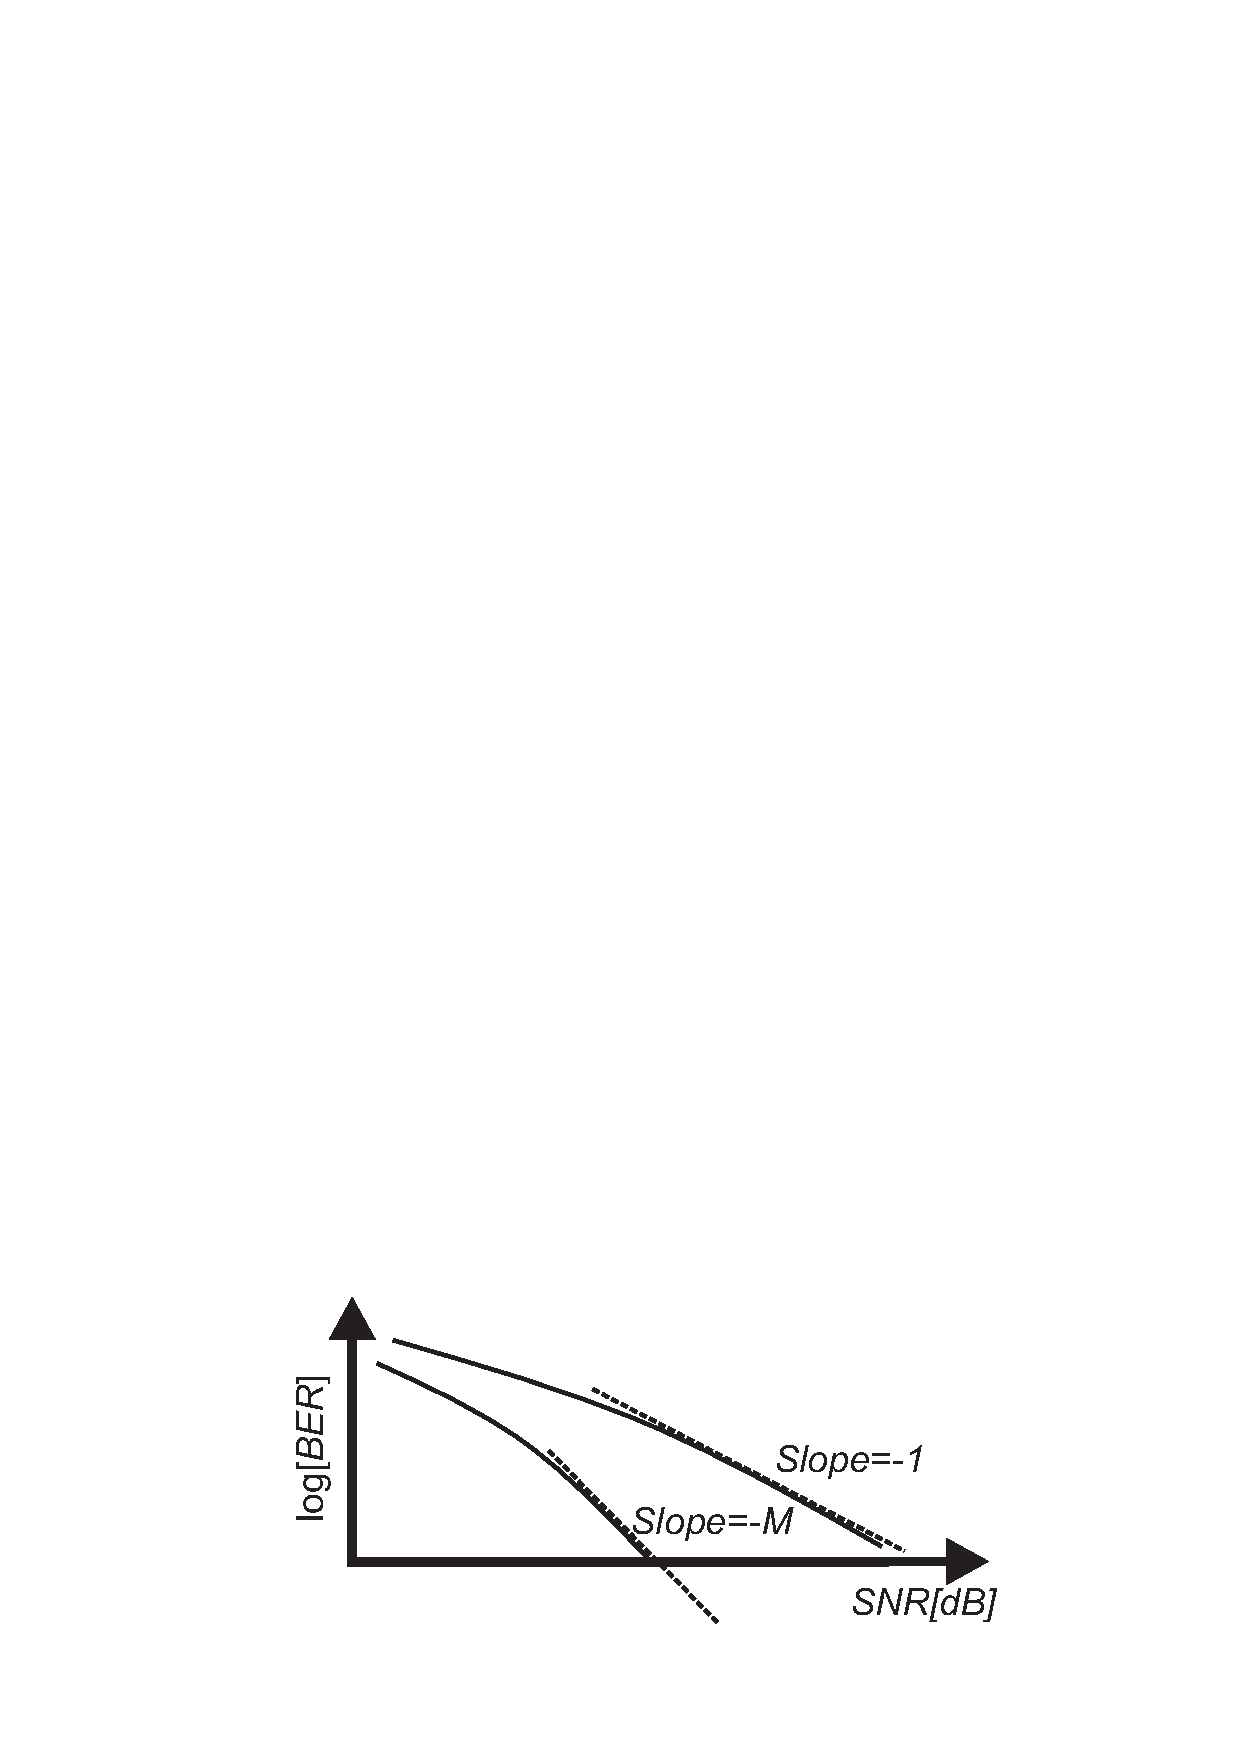
\includegraphics[width=6cm]{./figures/C02-alamouti_chart}
        \caption{Ganancia de diversidad espacio-tiempo en sistemas MIMO}
        \label{fig:alamouti_chart}
\end{figure}

Uno de los ejemplos más claros de \textit{space-time block coding} es el conocido como código de Alamouti. El código de Alamouti es un space-time block code ortogonal (O-STBC). Es implementado utilizando dos antenas en el transmisor y un número arbitrario de antenas en el receptor. Las palabras del código para múltiples antenas son escritas de la siguiente forma:

\begin{equation}
X = \frac{1}{\sqrt{2}}
\left( \begin{array}{cc}
\chi_1 & -\chi_2^* \\
\chi_2 & \chi_1^* \end{array} \right)
\end{equation}

El transmisor de Alamouti se muestra en la \ref{fig:alamouti}. El código de Alamouti tiene un rango de spatial multiplexing igual a uno, dado que se transmiten dos símbolos en el tiempo de duración de dos símbolos.

\begin{figure}[htb!]
        \centering
        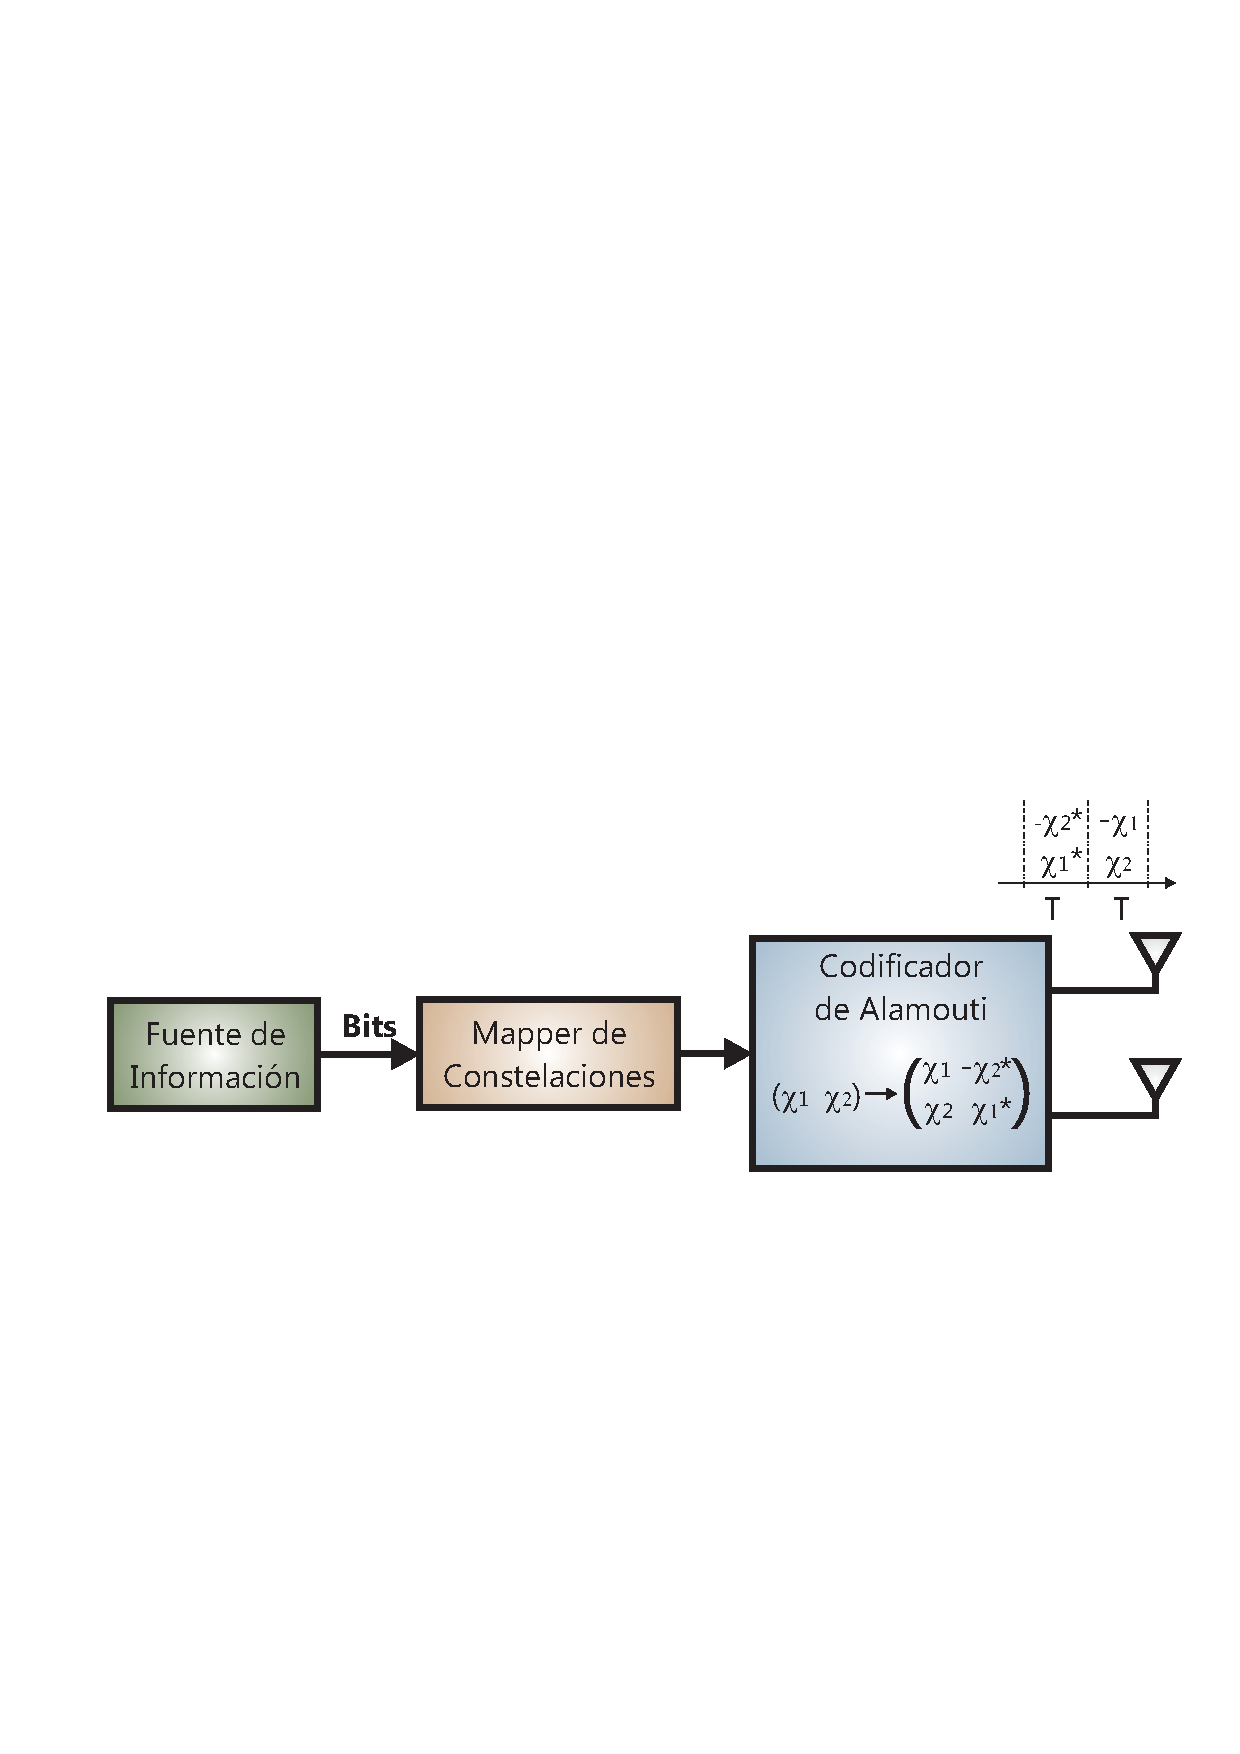
\includegraphics[width=10cm]{./figures/C02-alamouti}
        \caption{Esquema de un transmisor de Alamouti}
        \label{fig:alamouti}
\end{figure}

\subsection{\textit{Spatial multiplexing}}

\textit{Spatial Multiplexing} es una de las técnicas que se encuentra en el grupo de los códigos de capas de espacio-tiempo \cite{Mohammadi2}. En la misma, la secuencia de información es dividida en subflujos precisos. Los subflujos donde se lleva a cabo el procesamiento son conocidos como capas. Debido a ello a esta se la conoce como técnica de capas de espacio tiempo (LAST: layer space-time technique). Como se observa en la figura \ref{fig:spatial_multi1}, se transmiten $M_T$ subflujos independientes a través de $M_T$ antenas. En esta técnica, el número de antenas receptoras debe ser igual o mayor al número de antenas transmisoras.

\begin{figure}[htb!]
        \centering
        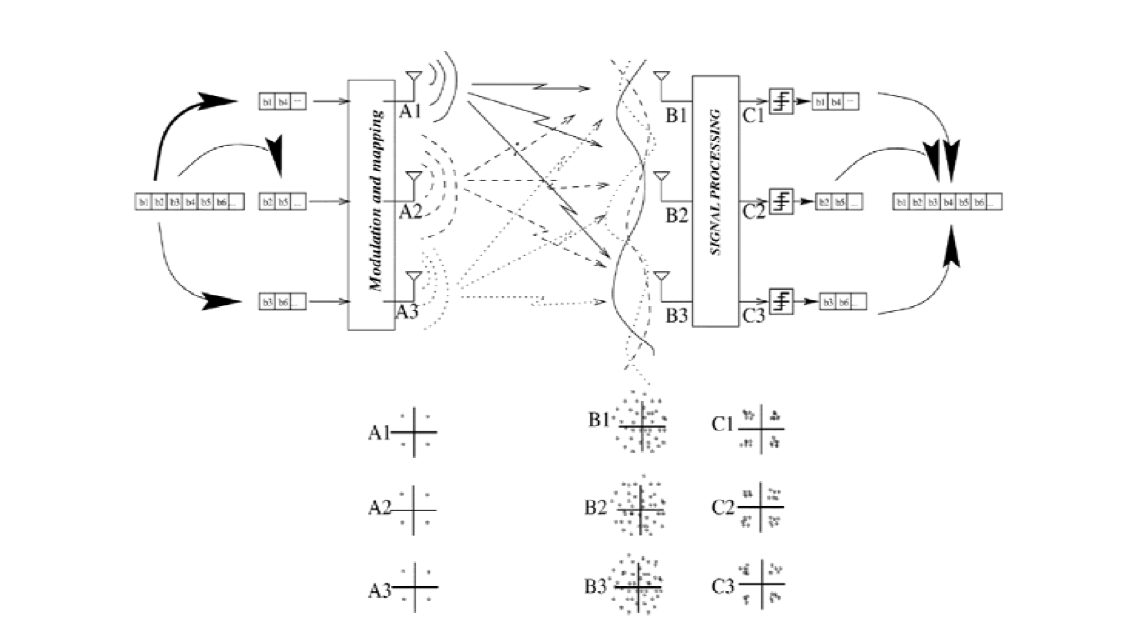
\includegraphics[width=13cm]{./figures/C02-spatial_multi_1}
        \caption{Spatial Multiplexing con tres antenas en transmisor y receptor}
        \label{fig:spatial_multi1}
\end{figure}

El proceso de dividir la secuencia de información en subflujos es realizado por un demultiplexor. El proceso de demultiplexado debe ser aplicado a bits o símbolos. Luego, la codificación puede ser realizada en tres formas diferentes de acuerdo a la posición del demultiplexor en la cadena del transmisor y la dirección de la capa. Estos procesos de codificación son referidos como horizontal, vertical y diagonal. Las distintas técnicas de codificación se muestran en la figura \ref{fig:spatial_multi2}.

\begin{figure}[htb!]
        \centering
        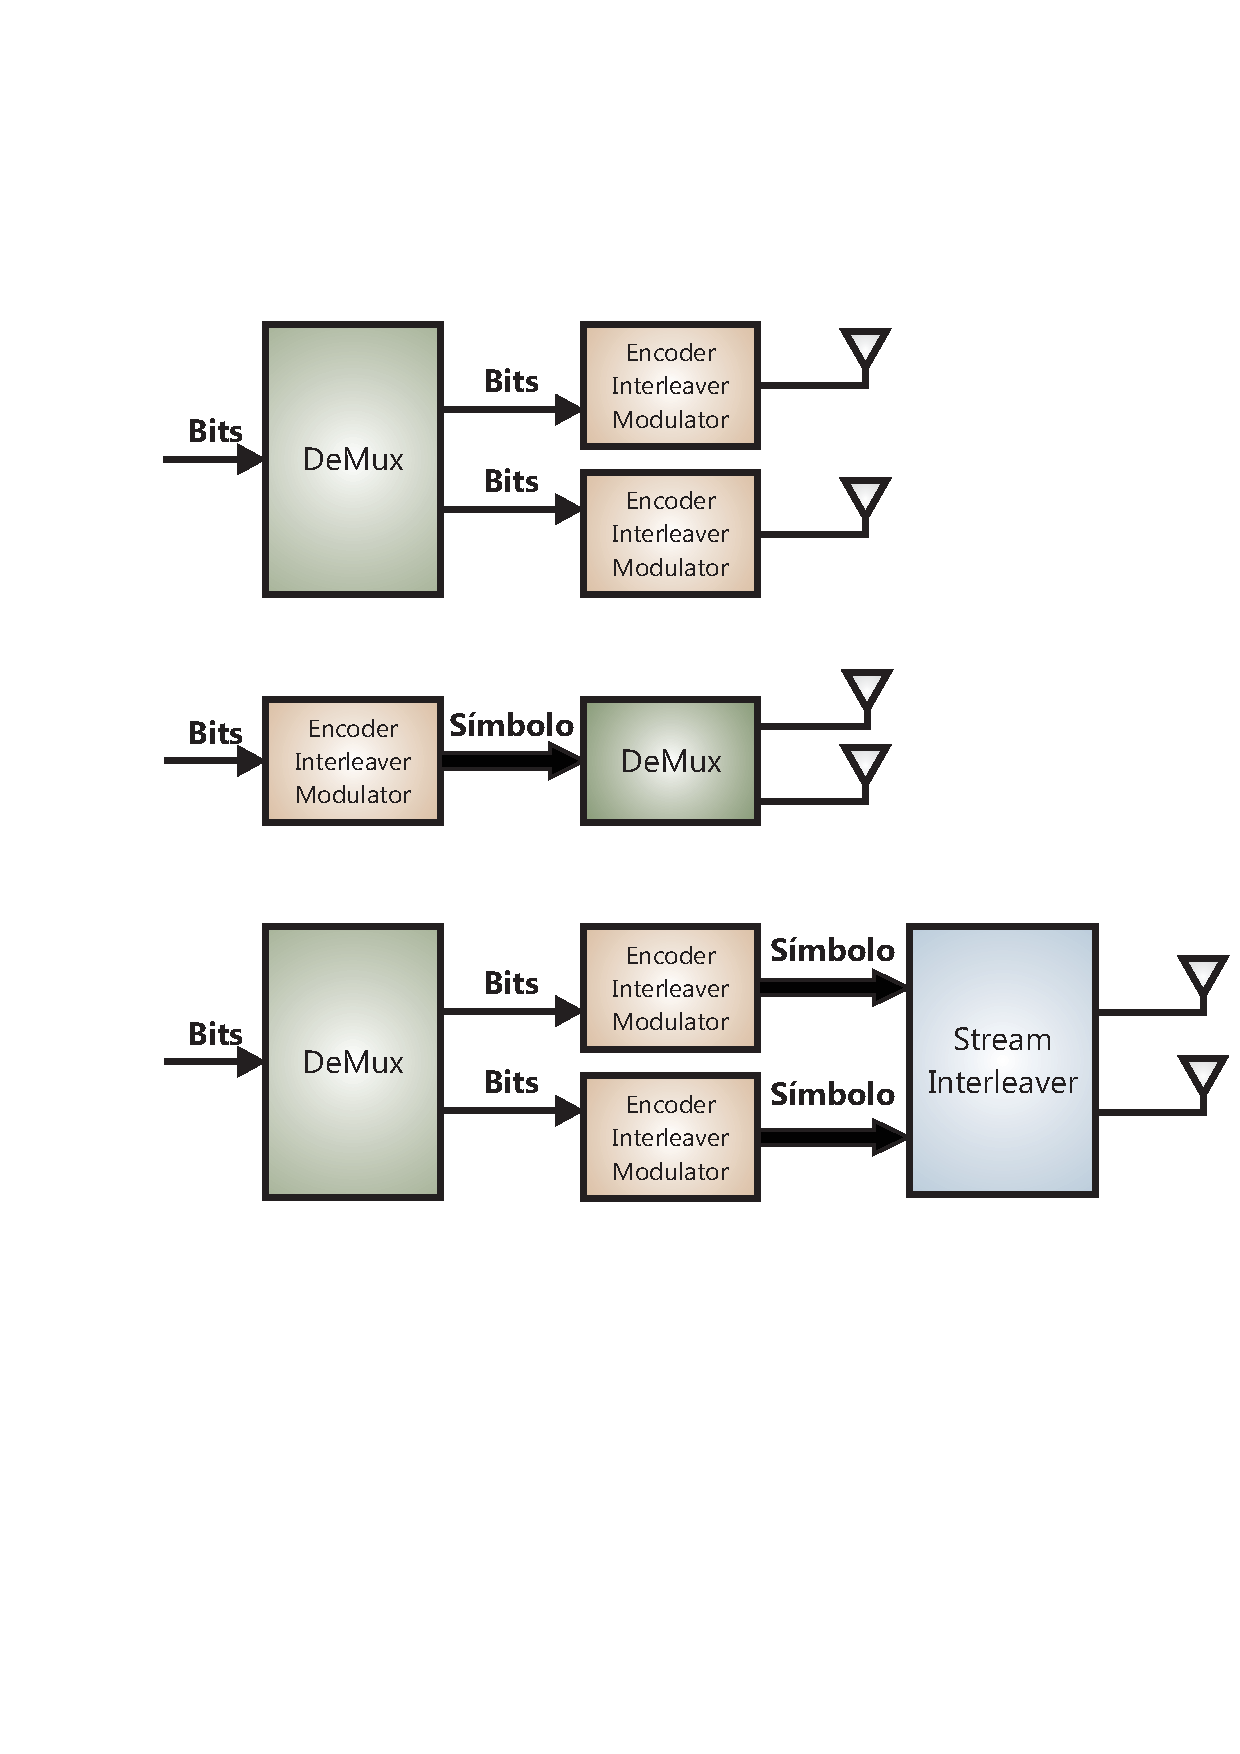
\includegraphics[width=9cm]{./figures/C02-spatial_multi2}
        \caption{Tipos de codificación para Spatial Multiplexing}
        \label{fig:spatial_multi2}
\end{figure}

\newpage

En el codificado horizontal, los bits de datos son demultiplexados en $M_T$ subflujos que son independientemente codificados, intercalados y modulados. Por otro lado, en la realización vertical, el flujo de datos es codificado, intercalado y modulado; y, los símbolos resultantes son luego demultiplexados en $M_T$ subflujos. El proceso para realizar spatial multiplexing diagonal es similar al codificado horizontal, con la única difrerencia de que, luedo de la etapa final, los frames de símbolos son sometidos a un intercalado de flujo, el cual rota los frames transmitidos.